\documentclass[oneside,12pt]{book}

% e-book format
\usepackage[paperwidth=210mm,paperheight=148mm,margin=10mm]{geometry}

% Cyrillization
\usepackage[T1,T2A]{fontenc}
\usepackage[utf8]{inputenc}
\usepackage[english,russian]{babel}
\usepackage{indentfirst}

% font setup for screen reading
\renewcommand{\familydefault}{\sfdefault}
\normalfont

% pdflatex options
\usepackage[unicode,colorlinks,linkcolor=blue,bookmarks=true]{hyperref}
\usepackage[pdftex]{graphicx}
\usepackage[usenames,dvipsnames,svgnames]{xcolor}

% listings
\usepackage{verbatim}
\usepackage{listings}
\lstset{
basicstyle=\small, % or \tiny \small or \footnotesize
extendedchars=true,inputencoding=utf8, % i18n
frame=single, % show frames around
numbers=left, numberstyle=\small,numbersep=1mm,% line numbering
tabsize=4, % tab style
keywordstyle=\color{Blue},%\texttt,
keywordstyle={[2]\color{Green}},%\texttt,
keywordstyle={[3]\color{Brown}},%\texttt,
keywordstyle={[4]\color{Red}},%\texttt,
keywordstyle={[5]\color{Blue}},%\texttt,
commentstyle=\color{Cyan}%\texttt%,
% showspaces=false
}

\usepackage{lstmk}\lstdefinestyle{mk}{language=mk}
\usepackage{lstrc}\lstdefinestyle{rc}{language=rc}

\newcommand{\lst}[3]{\lstinputlisting[title=\href{#2}{#1}]{#3}}
\newcommand{\lstx}[4]{\lstinputlisting[title=\href{#2}{#1},language=#4]{#3}}

% software menu & keys
\usepackage[os=win]{menukeys} 
\usepackage{amssymb} % windows key
\newcommand{\winstart}{$\boxplus$}
\newcommand{\winr}{\keys{\winstart+R}}
\newcommand{\file}[1]{\textbf{\textsf{#1}}}
\newcommand{\lms}{$\lhd$}
\newcommand{\dblms}{$\lhd\lhd$}
\newcommand{\rms}{$\rhd$}
\newcommand{\checkbox}{$\boxtimes$}
\newcommand{\uncheckbox}{$\square$}

% disable oneliner page breaks
\usepackage[defaultlines=2,all]{nowidow}

% books bib management
\usepackage{biblatex}
\addbibresource{../bib/python.bib}
\addbibresource{../bib/eskd.bib}
\addbibresource{../bib/electronics.bib}
\addbibresource{../bib/latex.bib}
\addbibresource{../bib/sat.bib}
\addbibresource{../bib/math.bib}
\addbibresource{../bib/sysdesign.bib}

\usepackage{makeidx}
\makeindex

% extra char sets
\usepackage{wasysym} % smileys

% set lists style
% \usepackage{enumitem}
% \setlist{nosep}

% misc

% \usepackage{titling}

\newcommand{\email}[1]{$<$\href{mailto:#1}{#1}$>$}
\newcommand{\internet}{Internet}

\newcommand{\cm}[1]{Cortex-M#1}
\newcommand{\cmx}{\cm{x}}

\newcommand{\linux}{Linux}
\newcommand{\emlinux}{em\linux}

\newcommand{\cpp}{$C^{+}_{+}$}
\newcommand{\py}{Python}

\newcommand{\vcs}{\hyperref[vcs]{VCS}}
\newcommand{\make}{\hyperref[make]{Make}}
\newcommand{\spice}{ngSPICE}
\newcommand{\latex}{\LaTeX}

\newcommand{\eclipse}{\textcircled{$\equiv$}\textsc{eclipse}}
\newcommand{\vim}{(g)Vim}

\newcommand{\note}[1]{\footnote{\ #1}}
\newcommand{\cp}[1]{\note{копипаста \url{#1}}}

\newcommand{\win}{\winstart Windows}

\newcommand{\mk}{МК}

\newcommand{\ram}{RAM}


\newcommand{\pref}[1]{/стр.\pageref{#1}/}

% selecting
\usepackage{framed}
\newcommand{\term}[1]{\textcolor{Green}{#1}}
\renewcommand{\emph}[1]{\textcolor{Blue}{#1}}
\newcommand{\prog}[1]{\textcolor{Brown}{#1}}
\newcommand{\pack}[1]{\textcolor{Magenta}{#1}}

% math
\usepackage{cancel}

% titles

\hypersetup{
	pdftitle={Азбука халтурщика-ARMатурщика},
	pdfauthor={ruOpenWrt, HackSpace <<Чебураторный завод>>, Консорциум хоббитов
	России, Bill Collis (Часть 1)}, 
	pdfsubject={https://github.com/ponyatov/Azbuka}
}


\begin{document}
\begin{titlepage}

\noindent

\includegraphics[height=0.4\textheight]{logo/CHBZ.png}
\hspace{1cm}

\includegraphics[height=0.15\textheight]{logo/LinuxPowered.png}
\hspace{1cm}
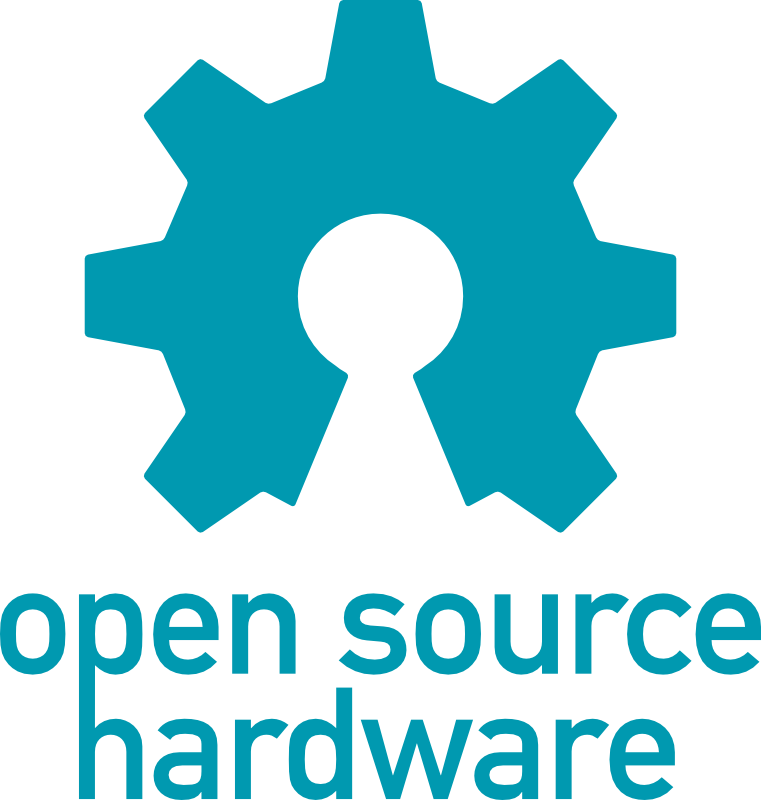
\includegraphics[height=0.4\textheight]{logo/OpenHardware.png}

\vspace{1.5cm}

\begin{centering}

{\Huge \textbf{\textsc{Азбука халтурщика-ARMатурщика \bigskip}}}

{\Huge \textbf{\textit{разработка встраиваемых систем}}}

{\Large 
основы бытовой автоматики,

систем управления и сбора данных
}

\end{centering}

\vspace{1cm}

{\large
\noindent
\copyright\
\href{https://groups.google.com/forum/\#!forum/openwrt2ru}{ruOpenWrt}
 \\
\copyright\
HackSpace
<<\href{https://github.com/ponyatov/CHBZ/raw/master/presentation.pdf}{Чебураторный
завод}>> \\
\copyright\
Консорциум хоббитов России
}
\end{titlepage}
\tableofcontents\clearpage

\clearpage\secly{О книге}

Эта книга\ --- комплект документации по аппаратно-программной платформе
ALYEH:

\begin{itemize}[nosep]
  \item \textcolor{red}{А}збука ARMатурщика
  \item \textcolor{red}{L}inux для встраиваемых систем
  \item д\textcolor{red}{Y}намический язык программирования \termdef{Ы}{Ы}
  \item библиотека \cpp\ для встраива\textcolor{red}{E}мых систем  
  \item \textcolor{red}{H}ardware библиотека универсальных модулей
\end{itemize}
\bigskip

\emph{В текущем состоянии эта книга\ --- конспект материалов, которые я сейчас
собираю, в черновой верстке. Объем материала очень большой, фактически это целая
специальность для приличного техникума, что-то типа ``Технология цифрового
производства''. Поэтому 146\% пока составляет сырая копипаста, с редкими
вкраплениями собственного бреда. В процессе адаптации, обкатки на студентах и
доработки эта поделка должна принять более вменяемый вид. Но учитывая полное
отсутствие обратной связи, этого никогда не случиться.}
\bigskip

Это учебное пособие было создано для интересующихся любительской электроникой,
самодельными цифровыми системами управления (Arduino, устройствами на
микроконтроллерах и т.п.), и программистов-лю\-би\-те\-лей. В связи с полной
деградацией системы образования пособие также рекомедуется для применения при
обучении в ВУЗах по специализациям, связанным с применением цифровой электроники
и компьютерной техники.

Большой упор был сделан на использование открытого некоммерческого программного
обеспечения, для удешевления учебного процесса, уменьшения себестоимости ваших
проектов\note{вряд ли ли у вас окажется лишняя пачка килобаксов на покупку пары
коммерческих САПР, по крайней мере пока ваш стартап не взлетит в Top\$100K}, и
стимулирования вашего участия в развитии этих программных пакетов.

Книга очень объемна и разнообразна по материалу, и построена как справочник с
группировкой материала по тематике. Для тех, кто только начинает, в разделе
\ref{learnplans}\ расписаны \termdef{пошаговые учебные планы}{учебный план} с
точки зрения параллельного изучения нескольких предметов с постепенным
усложнением\note{как это происходит при традиционном offline обучении}. Как
известно, главная часть любого обучения\ --- практическая. Особое внимание
уделено набору лабораторных работ.

\bigskip
В качестве видеоматериала были использованы 
\href{https://www.youtube.com/playlist?list=PLddc343N7YqgCWlspw08g6t0iFos9gAi4}{видеоуроки
физики}\\
\copyright\ Ерюткин Е.С., учитель физики высшей категории 
\href{http://sch1360v.mskobr.ru/}{ГБОУ СОШ №1360}, г.Москва

\bigskip
Мы признательны Bill Collis за разрешение использовать материалы его книги
<<\href{www.techideas.co.nz}{An Introduction to
Practical Electronics,
Microcontrollers and
Software Design}>> \cite{bcollis} в
русскоязычном варианте <<Азбуки>> (\ref{bcollis}), и конечно он вполне
заслуженно включен в основные соавторы этой книги.

\bigskip
Так как для работы в области электроники необходимо владение технологиями
изготовления конструктива, в книгу включен соответствующий раздел. 
Эти книги рекомендуются популярным поставщиком хоббийных настольных
микро-станков \href{http://sherline.com/}{Sherline Products}. Так как от
владельцев авторских прав не получено разрешение на полный официальный перевод,
для этих книг сделан только перевод-подстрочник, который поможет вам читать
оригинал:
\begin{itemize}
  \item Joe Martin, Craig Libuse \textbf{Tabletop Machining}
  \cite{tabletop} (\ref{tabletop})
  \item Doug Briney \textbf{Home Machinists Handbook}
  \cite{briney} (\ref{briney})
\end{itemize}

Отечественных книг по использованию маленьких ``часовых'' и настольных станков
просто не существует, хотя они и выпускались серийно. Исключение\ --- книга
Евгений Васильев \textbf{Маленькие станки} \cite{vasil}, но она имеет обзорный
характер.

\bigskip
\textbf{Лицензия на эту книгу пока не выбрана, так что она пока просто пишется в
духе OpenSource: любой может использовать ее часть, изменять или дополнять, до
тех пор, пока не накладываются какие-либо административные, финансовые или
юридические ограничения на распространение и развитие оригинальной версии или ее
открытых форков: \url{https://github.com/ponyatov/A}}
\bigskip

Приглашаем всех желающих участвовать в развитии этого учебного пособия на форум
\href{https://groups.google.com/forum/\#!forum/openwrt2ru}{ruOpenWrt} и в группу
\url{http://vk.com/samarahackerspace}, нам нужна обратная связь по качеству
материала, результаты тестирования на вас или ваших студентах, дополнения и
замечания.


\part{Основы электроники}

Здесь идет список ссылок на онлайн лекции в edX, Coursera, и т.п.

\chapter{Линейные схемы на пассивных элементах, основы электротехники}

\chapter{Симуляция и расчет схем в \spice}

\chapter{KiCAD}

\cp{http://teholabs.com/knowledge/kicad.html}

\noindent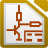
\includegraphics[height=0.5\textheight]{tmp/icon_kicad.png}


\cp{http://ru.wikibooks.org/wiki/KiCad}

KiCad\ --- распространяемый по лицензии GNU GPL программный комплекс САПР EDA с
открытыми исходными текстами, предназначенный для разработки электрических схем
и печатных плат.

Кроссплатформенность компонентов KiCad обеспечивается использованием 
библиотеки wxWidgets. Поддерживаются операционные системы Linux, 
Windows NT 5.x, Free\-BSD и Solaris.

Разработчик\ --- Жан-Пьер Шарра (фр. Jean-Pierre Charras), исследователь 
в LIS (фр. Laboratoire des Images et des Signaux\ --- Лаборатория Изображений 
и Сигналов) и преподаватель электроники и обработки изображений в фр. 
IUT de Saint Martin d’Hères (Франция).

\cp{http://ru.wikibooks.org/wiki/KiCad/Miniurok}

Этот раздел познакомит Вас с основами использования системы KiCad. Он содержит
информацию о всех шагах создания простой печатной платы: от рисования
электрической схемы до печати готового рисунка платы. Вам будут представлены
различные возможности KiCad и предложены эффективные пути решения различных
задач.

Руководство пользователя, поставляемое вместе с KiCad, содержит значительно
больше информации, чем этот урок. Ознакомтесь с ним, чтобы узнать больше об
использовании программы.



\secrel{Установка}\secdown

\secrel{\win}\label{kicadinstwin}

\menu{\winr{\url{http://www.kicad-pcb.org/}}>Download>\winstart}

\menu{\winr{\url{http://kicad.nosoftware.cz/}}>
\file{KiCad\_testing\-201x.xx.xx-BZRxxxx\_Win\_full\_version.exe}}

\bigskip

\menu{Installer Language>\emph{English}>Ok} 
в русифицированном инсталляторе кривые шрифты

\menu{KiCAD 20xx.xx.xx Setup>Next}

\menu{Лицензия>Agree}

\menu{Components>\checkbox\ все>Next}

\menu{Location>\file{C:/KiCad}>Install}

\menu{Completing Setup>\uncheckbox Wings3D>Finish}

\secrel{\linux}\label{kicadinstlin}

\begin{verbatim}
root# aptitude install kicad-doc-ru kicad
\end{verbatim}

\lst{+++\ $\sim$/.blackbox/menu}{}{/tmp/kicad.bbmenu}

\secrel{Настройка библиотек}

Для добавления библиотек, поставляемых с этой книгой, сделайте \emph{git
clone} или \emph{git pull}:

\begin{verbatim}
user:~$ git clone --depth=1 -o gh https://github.com/ponyatov/odurino.git odurino
user:~$ cd odurino
user:~/odurino$ git pull
\end{verbatim}

\menu{\prog{kicad}>\prog{eeschema}>Настройки>Библиотека}

\menu{Пользовательские пути поиска>Добавить>\file{/home/user/odurino/lib}}

\menu{Файлы библиотек>все стандартные>Удалить>OK}

\menu{Файлы библиотек>Добавить>R,L,C,SPICE,DA\_POWER,..>Открыть>OK}

\bigskip
Для проверки работы библиотек можете открыть проект

\menu{\prog{kicad}>Файл>Открыть>\file{~/Azbuka/bcollis/led1/led1.pro}}

или сразу схему

\menu{\prog{eeschema}>Файл>Открыть>\file{~/Azbuka/bcollis/led1/led1.sch}}

\secrel{Дотфайлы}

Посколько программа изначально писалась как юниксовая, пользовательские
настройки хранятся в dot-файлах:

\lst{~/.kicad}{}{kicad/kicad.dotfile}

\begin{description}
\item[KicadFrame*] размеры и положение окна менеджера проектов
\item[WorkingDir] каталог с текущим рабочим проектом
\item[fileN] список последних проектов (\ \menu{Файл>Последние файлы}\ )
\end{description}

\lst{~/.eeschema}{}{kicad/eeschema.dotfile}

\begin{description}
\item[SchematicFrame*] размеры и положение окна \prog{eeschema}
\item[fileN] список последних схем (\ \menu{Файл>Последние файлы}\ )
\end{description}

\secrel{Глобальные шаблоны}\label{kicadtemplates}

После установки \kicad\ можно скорректировать файлы глобальных шаблонов, чтобы
новые проекты создавались сразу с нужными настройками, прежде всего с нужным
нам набором библиотек:

\begin{verbatim}
sudo vim /usr/share/kicad/template/kicad.pro
\end{verbatim}

\lst{/usr/share/kicad/template/kicad.pro}{}{kicad/kicad.template}

\begin{description}
\item[LibDir] каталог библиотек, установите на свой или корпоративный/групповой
\item[LibNameN] задается список библиотек по умолчанию, приопишите ваш типовой
набор
\item[eeschema/libraries] схемные библиотеки \eeschema
\item[pcbnew/libraries] библиотеки надстеков для печатных плат \pcbnew
\end{description}

\secup


\section{Создание проекта в менеджере проектов \prog{kicad}}

В верхней части панели \term{менеджера проектов} \prog{kicad}
имеются большие кнопки запуска компонентов KiCad:

\begin{itemize}
\item \icoesch\ \prog{EeSchema}\ --- Редактор принципиальных схем
\item
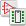
\includegraphics[height=0.1\textheight]{tmp/icon_cvpcb.png}\
\prog{CvPcb}\
--- Программа редактирования падстеков (отверстий и площадок)
\item 
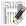
\includegraphics[height=0.1\textheight]{tmp/icon_pcbnew.png}
\prog{Pcbnew}\ ---
Редактор печатных плат
\item
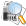
\includegraphics[height=0.1\textheight]{tmp/icon_gerbview.png}
\prog{GerbView}\ --- Программа просмотра фотошаблонов в формате Gerber
\item \prog{Bitmap2Component}\ --- Создание компонента из черно-белого
изображения (например логотипа)
\item 
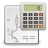
\includegraphics[height=0.1\textheight]{tmp/icon_pcbcalculator.png}
\prog{PcbCalculator}\ --- Калькулятор для печатных плат
\item 
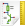
\includegraphics[height=0.1\textheight]{tmp/icon_pagelayout.png}
\prog{PageLayout}\ --- редактор формата листа схемы
\end{itemize}

Каждая кнопка запускает соответствующую программу. Мы будем использовать эти
программы по мере изучения.

\bigskip
Лучше всего для каждого проекта использовать раздельные папки; в противном
случае система может сбиться с толку, если файлы из разных проектов будут лежать
в одной папке. Проделайте следующие шаги:

\begin{enumerate}
  \item Создайте папку проекта \file{D:/ARM/SpindleDriver}
  \item Запустите программу KiCad
  \item Создайте проект (project)
  \begin{itemize}
    \item 
На панели инструментов KiCad выберите левую иконку с подсказкой\\
\menu{Начать новый проект}, используйте команду меню
\menu{Файл>Новый>Пустой} или сочетание клавиш \keys{Ctrl+N}.
    \item 
В диалоге \menu{Создать новый проект} выберите созданную папку
выберите только что созданную папку \file{D:/ARM/SpindleDriver} и
введите имя проекта \menu{\file{SpindleDriver}} и нажмите \menu{Сохранить}.
	\item
Если папка проекта содержит какие-то файлы, будет выведено окно выбора:
создать подпапку с именем проекта \menu{Yes}, или записать файл проекта
в указанную папку как есть \menu{No}. Нажмите No.
    \item 
Сохраните проект кнопкой \menu{Сохранить текущий проект}, \menu{Файл>Сохранить}
или \keys{Ctrl+S}.
	\item
В папке появится файл \file{SpindleDriver.pro}, содержащий установки вашего 
проекта. Файл имеет тектовый формат, поэтому при необходимости его можно открыть
в любом редакторе и вручную аккуратно подправить, например скорректировать
настройки зазоров печатной платы.
  \end{itemize}
\end{enumerate}

\section{Создание принципиальной схемы в \prog{eeschema}\ (часть 1)}

Запустите редактор принципиальных схем, нажав на панели KiCad большую кнопку
\icoesch.

При первом запуске \prog{eeschema}\ стартует с новым проектом и
показывает предупреждение, что файла схемы еще нет. Просто нажмите \menu{ОК}.

Если вас не устраивает черный фон рабочец области или цвета элементов схемы,
поменяйте настроки цветов \menu{Настройки>Цвета}. 

На правом краю окна редактора схем есть вертикальная панель инструментов,
которые мы и будем использовать для рисования схемы. Этими инструментами можно
выбирать объекты, размещать компоненты, вводить связи и т.д.

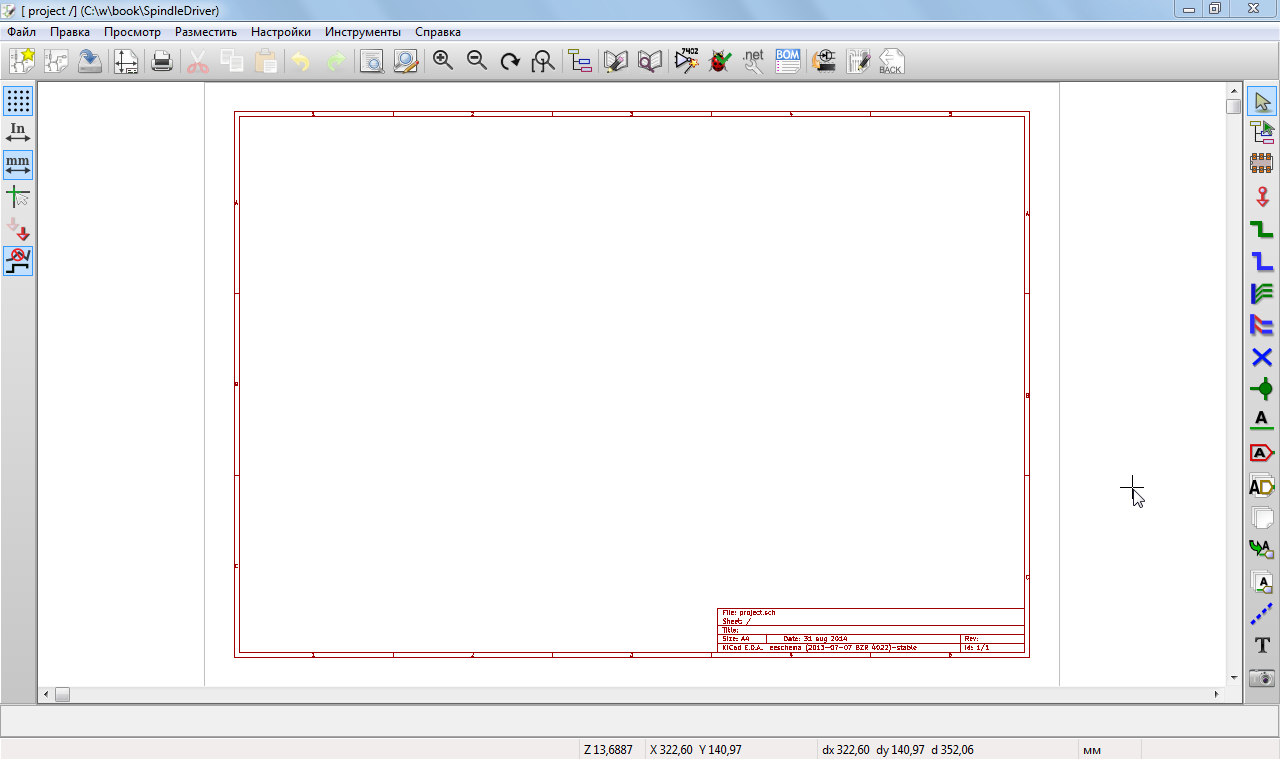
\includegraphics[width=0.9\textwidth]{kicad/ee15.png}

Завершение работы инструмента: вы можете выбрать другой инструмент из правой
инструментальной панели или же указать \menu{Отложить инструмент} по правому
клику мышки \keys{\rms}.

\section{Инструмент \emph{Добавить компоненты}}

\begin{itemize}
  \item 
На правой панели нажмите кнопку \menu{Разместить компонент}\
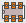
\includegraphics[height=2em]{kicad/ee21.png}. Курсор изменится со стрелки на
карандаш. Удобнее использовать сочетание клавиш \keys{Shift+A}.
Кликните в поле схемы чтобы начать размещение компонента. Появится диалог
\menu{Выбор компонента}. Вы можете выбрать компонент несколькими путями:
  \item
  \begin{enumerate}
    \item 
Если вы знаете точное имя копонента, введите его в поле \menu{Имя}, а
затем нажмите \keys{Enter} или \keys{OK}.
    \item 
Если вы знаете имя только приблизительно, в поле \menu{Имя} введите шаблон для
поиска, например, \menu{*BD*}, затем нажмите \keys{Enter} или \keys{OK}. Вы
увидите окно \\\menu{Выбрать компонент} со списком найденных компонентов.

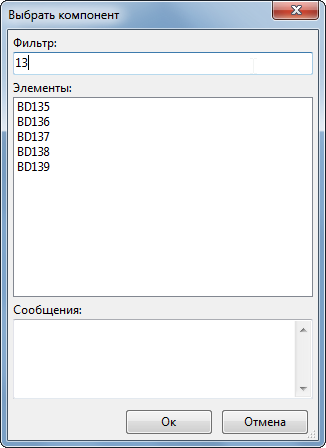
\includegraphics[height=0.5\textheight]{kicad/ee16.png}
    \item 
Вы можете искать компонент по ключевому слову, введя его в поле \menu{Имя},
затем кликнув \menu{Поиск по ключевому слову}. Однако на данный момент качество
библиотек все еще низкое, и немногие компоненты имеют ключевые слова, поэтому
эта возможность полезна косвенно.
    \item 
Можно выбрать недавно использованные компоненты из \menu{Списка истории}.
    \item 
Кнопка \menu{Список всех} вызывает диалог, в котором можно выбрать сначала
библиотеку \menu{74xx}, а затем ее компонент \menu{74HCT04}.
    \item 
Кнопка \menu{Выбор просмотром} вызывает \menu{Обзор библиотек}, позволяя
просмотреть библиотеки и находящиеся в них условные графические изображения.

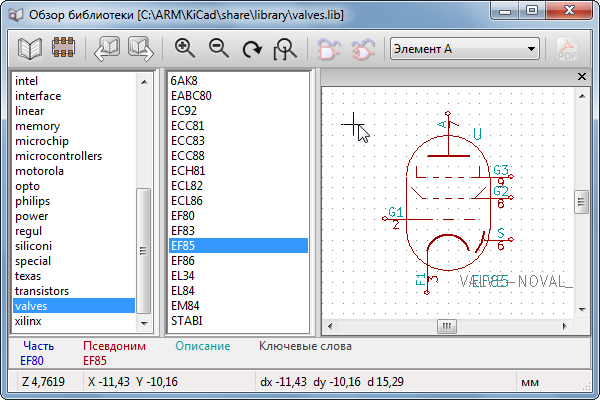
\includegraphics[height=0.5\textheight]{kicad/ee19.png}

  \end{enumerate} 
\end{itemize}

Вы также можете
вызвать обозреватель библиотек кнопкой\\
\menu{Просмотр библиотек и
компонентов}\ 
\includegraphics[height=2em]{kicad/ee20.png}

Выбрав элемент \dblms, вставьте символ в нужное место схемы \lms.
Позже вы сможете переместить его если нужно.
Зеркальное отражение компонента можно произвести следующим образом:

\begin{itemize}
  \item Поместите курсор на компоненте.
  \item По \rms\ выберите \menu{Ориентация компонента>Отражение}. 
  \item Без использования \term{контекстного меню}\ --- наведите мышь на
  компонент и нажмите кнопку \keys{X}\ или \keys{Y}.
\end{itemize}




\secrel{\prog{eeschema}: редактор электрических схем}

обеспечивает:

\begin{itemize}
\item создание однолистовых и иерархических схем,
\item проверку их корректности ERC (контроль электрических правил),
\item создание списка электрических цепей netlist для редактора топологии платы
pcbnew или для spice-моделирования схемы, 
\item доступ к документации на используемые в схеме электронные компоненты
(datasheet).
\end{itemize}


\secrel{Библиотеки компонентов}\secdown

\cp{http://habrahabr.ru/post/197582/}\bigskip

Модель компонента в САПР EDA состоит из следующих частей:

\begin{itemize}
  \item условное графическое обозначение (УГО) для схемного редактора
  \item модель компонента для редактора печатных плат (ПП)
  \item модель для симулятора (SPICE)
  \item 3D модель для передачи в универсальный САПР для работы с конструкцией
  \item дополнительные пользовательские данные: индексы компонента для
  заказа у разных поставщиков, ссылки на документацию, и т.п.
\end{itemize}

Части могут иметь несколько вариантов, например два варианта УГО (ГОСТ и ISO),
три корпуса (DIP, PLCC и LQFP), две модели для симулятора (идеальная и с
учетом паразитных эффектов), и 2 механических модели (габаритный кубик, и
подробная).

Кроме того, часто в один корпус упаковывается несколько одинаковых или разных
элементов. Одинаковые\ --- 2--4 операционных усилителя (ОУ), или вентили
логики. Разные\ --- части вакуумной лампы, разнесенные на схеме по разным
каскадам.

\bigskip

В составе KiCad поставляются библиотеки электронных компонентов (обычных и
поверхностно монтируемых SMD). Для многих библиотечных компонентов есть
3D-модели, созданные в \prog{Wings3D}.

Но как только вы начинаете работать со свежеустановленным KiCADом, тут же
обнаруживается, что библиотечные компоненты или не подходят\note{например не
соответствуют ГОСТ или стандартам предприятия}, или нужных компонентов попросту
нет в библиотеках.

Рассмотрим последовательное создание совершенно нового элемента на примере
модуля USB интерфейса HEX\_FT2232RL \ref{HEXFT2232RL}

\secrel{Создание УГО для схем}

Нам необходим встроенный редактор символов схем (библиотечных компонентов),
запускаем его следующим образом:

\begin{enumerate}
  \item Вначале запускаем \file{eeschema}
  \begin{itemize}
    \item[вверху] меню и панель инструментов
    \item[слева] область размерности и шага сетки редактора (настройка рабочей
    области)
    \item[справа] область элементов схем и перемещения по иерархии схемы
  \end{itemize}
  \item Далее запускаем встроенный
  \menu{Редактор библиотек}\ 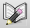
\includegraphics[height=2em]{kicad/ee22.png}

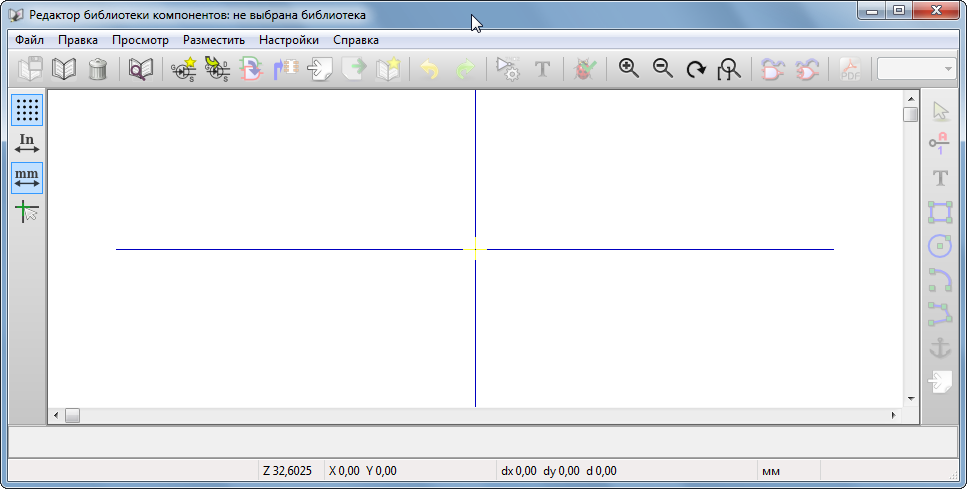
\includegraphics[height=0.5\textheight]{kicad/lib23.png}
\end{enumerate}

Необходимо создать новую библиотеку и первый собственный компонент:

\menu{Создать новый компонент}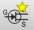
\includegraphics[height=2em]{kicad/newel.png},

\menu{Свойства компонента>Общие Настройки},

\menu{Имя компонента>HEX\_FT232RL}

\menu{Обозначение по умолчанию>U}

\menu{Количество элементов в корпусе>1}

\menu{OK}
\bigskip

В верхней панели инструментов активировались несколько кнопок, выбираем

\menu{Сохранить текущий компонент в новой библиотеке}

\includegraphics[height=2em]{kicad/lib26.png}

В открывшемся диалоге выберите каталог для библиотеки
\file{/home/user/kicad/}, и укажите имя файла (новой) библиотеки
\menu{\file{MyModules}>Сохранить}.

\bigskip
Теперь нужно добавить созданную библиотеку в рабочий список.
\bigskip

Настроим дополнительный путь, где лежат файлы библиотек. Это могут быть ваши
личные библиотеки, специальная библиотека для конкретного проекта, или комплект
библиотек поставляемых вместе с этой книгой: выберите в меню
\menu{Настройки>Библиотека}, \menu{Пользовательские пути
поиска>добавить>\file{/home/user/kicad/}}, \menu{Ok}.

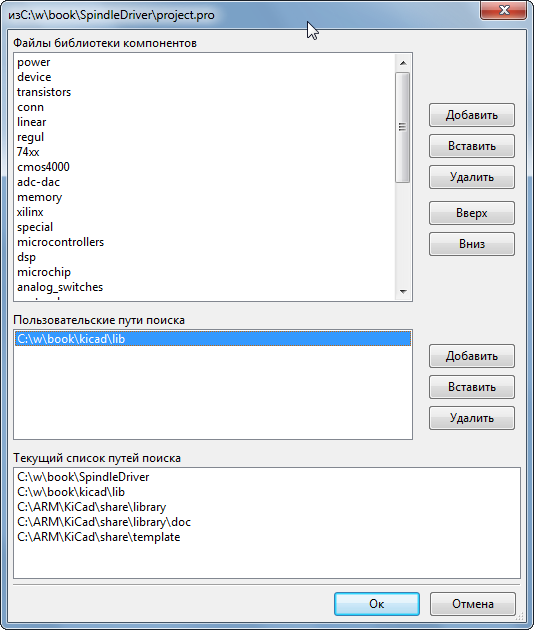
\includegraphics[height=0.5\textheight]{kicad/lib25.png}

\menu{Настройки>Библиотека},
\menu{Файлы библиотеки компонентов>power>\lms>Вставить}.
Выбираем только что созданную библиотеку \file{MyModules}.
Она будет вставлена в список до выбранной \file{power}.

\bigskip
Проделанные настройки применятся только к текущему проекту. Если Вы хотите 
чтобы новая библиотека всегда добавлялась к новым проектам, вам нужно добавить
новый путь поиска библиотек и ее название в файл шаблона, как это описано в
\ref{kicadtemplates}.

\bigskip
Если вы хотите изменить только что созданное или уже сущесствующее УГО, нужно
выбрать рабочую библиотеку, ту библиотеку в которой мы хотим работать (создавать
или редактировать компоненты). На панели инструментов нажимается кнопка

\menu{Выбор рабочей библиотеки}
\includegraphics[height=2em]{kicad/lib24.png},

\menu{Выбрать библиотеку>MyModules>Ok}.

Загружаем созданный ранее (пустой) компонент \file{HEX\_FT232RL} (или любой
другой)

\menu{Загрузить компонент для редактирования}
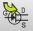
\includegraphics[height=2em]{kicad/editel.png}

\menu{Выбор компонента>Список всех>Элементы>\file{HEX\_FT232RL}>Ok}

\bigskip
\includegraphics[height=0.45\textheight]{odurino/usb/HEXFT232RL.png}

Сейчас у нас элемент не имеет графических элементов, и состоит только из
нескольких текстовых полей с обозначениями, слепленных в одной точке. Нужно их
растащить: \rms, САПР не может различить близкие элементы и уточняет для
какого поля мы хотим контекстное меню. Выбираем любое, \menu{Переместить поле}\
или кнопка \keys{M}. Перетаскиваем элемент, и \lms\ на свободном месте.

Пользуясь \ref{eskd}, отрисовываем на освободившемся месте УГО элемента,
пользуясь кнопками на панели справа. Рисование выполняется по сетке, шаг
выбирается \menu{\rms>Выбор сетки}, набор сеток фиксированный (?). При рисовании
ГОСТовских УГО округляем до ближайших дюймовых размеров\footnote{\ 1mil=1/1000
дюйма, 100mil=2.54mm=типовой шаг DIP микросхем}, или в меньшей сетке если нужно
точно гостовские размеры.

УГО имеет \term{точку привязки}, относительно которой отрисовываются элементы.
На практике важно то, что вокруг этой точки элемент вращается. Для перемещения
этой точки можно использовать кнопку

\menu{Переместить точку привязки}
\includegraphics[height=2em]{kicad/lib27.png}.

Добавляем выводы компонента: \menu{Добавить вывод
компонента}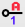
\includegraphics[height=2em]{kicad/lib28.png}.

\bigskip
Например для резистора создание выводов будет выглядеть вот так:

\bigskip
\menu{Свойства вывода}

\menu{Имя>A}

\menu{Номер>1}

\menu{Ориентация>Вправо}

\menu{Электр.тип>Пассивный}

\menu{Размер шрифта>1.27мм}

\menu{Длина>2.54мм}

\menu{Ok}

\bigskip

\menu{Имя>B}

\menu{Номер>2}

\menu{Ориентация>Влево}

\menu{Ok}

\bigskip
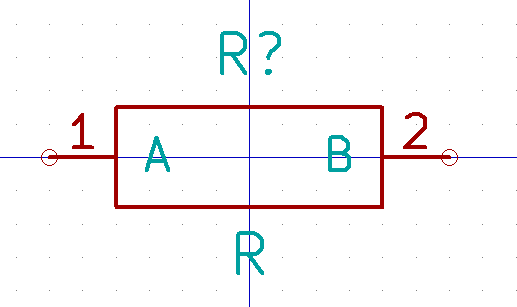
\includegraphics[height=0.5\textheight]{kicad/lib29.png}
\bigskip

Сохраняем библиотеку: \menu{Сохранить текущую
библиотеку}
\includegraphics[height=2em]{kicad/lib30.png}

\menu{Подтверждение>Включая последние изменения компонента?>Да}

\menu{Подтверждение>Компонент существует. Изменить его?>Да}

\menu{Подтверждение>Изменить файл библиотеки ?>Да}

\secrel{Модель печатной платы}

Модель печатной платы в программе \pcbnew\ состоит из нескольких
\termdef{слоев}{слой печатной платы} с разными функциями, для типичной
двухслойной ПП:

\begin{itemize}
  \item верх
  \begin{description}
  \item[Front] медь верхнего слоя
  \item[Adhes\_Front] карта нанесения клея для компонентов
  \item[SoldP\_] карта нанесения паяльной пасты
  \item[SilkS\_] шелкография: маркировка элементов, надписи, и т.п.
  \item[Mask\_] паяльная маска 
  \end{description}
  \item низ
  \begin{description}
  \item[Back] медь нижнего слоя
  \item[Adhes\_Back] карта нанесения клея для компонентов 
  \end{description}
  \item контуры
  \begin{description}
  \item[Контур ПП] слой определяющий физ.геометрию платы, используется при
  фрезеровке контуров, сверлении монтажных отверстий, разделке сверловкой и т.п.
  \item[Пояснения] вспомогательная текстовая информация
  \item[Чертеж] вспомогательная графическая информация: габаритные размеры, зоны
  монтажа,..
  \end{description}

\item В зависимости от технологии производства и пожеланий разработчика могут
добавляться любые дополнительные слои.
\end{itemize}

\secrel{Создание падстека}

\termdef{Падстек}{падстек}\ --- модель контактной площадки компонента, в виде
набора геометрий отдельно для каждого \term{слоя} печатной платы. Также включает
информацию о диаметре сверления.

% \secrel{PS:}
% 
% Компоненты и посадочные места корпусов можно ассоциировать с документацией,
% ключевыми словами и осуществлять быстрый поиск компонента по функциональному
% назначению.
% 
% \secup
% 
% \secru{Отрисовка схемы (часть 2)}
% 
% \secdown
% 
% \secru{Автоматическое обозначение элементов}
% 
% Автоматическое обозначение элементов и перенумерация выполняется кнопкой\\
% \menu{Обозначить компоненты на
% схеме}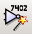
\includegraphics[height=2em]{kicad/ee000004.png}
% 
% \secru{Генерация списка цепей}
% 
% Список цепей (нетлист) используется для передачи информации о соединении
% компонентов между программами. Чаще всего СЦ создается после отрисовки схемы для
% передачи данных в программу трассировки печатной платы (ПП).

\secup


\secrel{\prog{gerbview}: просмотр фотошаблонов}

позволяет просматривать Gerber-файлы перед передачей печатных плат в
производство.


\section{Программа \prog{Wings3D} для создания 3D моделей}

Эта программа может вам пригодиться если вы планируете создавать 3D модели для PCB элементов.

Архив и файлы документации (Linux и Windows) в папке kicad/wings3d.

Взгляните на домашнюю страницу Wings3D чтобы узнать подробнее о программе.

pcbnew использует файлы в формате wrml (.wrl) экспортируемые из Wings3D (родной формат Wings3D - это .wings).

\subsection{Установка \prog{Wings3D} под \win}

\menu{\winr{\url{http://www.wings3d.com/}}>Downloads>Stable Release>\win
(32/64b)}

\menu{file{wings-n.n.n.exe}}

\menu{Compononets>\checkbox QuickLaunch>Next}

\menu{Location>\file{C:/Program Files/wings3d\_n.n.n}>Next>Install>Close}% 



\chapter{Простейшие полупроводниковые элементы}

\section{Оптоэлектроника}

\section{Схемы на биполярных транзисорах} 

\section{Схемы на на полевых транзисорах}

\chapter{Операционные усилители}

\chapter{Источники питания}

\section{Батарейное питание}

\section{Линейные стабилизаторы}

\section{Импульсные преобразователи на ШИМ-контроллерах} 

\section{Цепи защиты и гашения кондуктивных помех}

\chapter{Цифровая электроника}

\chapter{Компьютерные интерфейсы}

\section{Поколение 90х: COM, LPT, ISA}

\subsection{Резервный программатор AVR ``пять проводков''}

\section{Сеть CAN}

\section{Интерфейсные модули USB}

\subsection{Универсальный высокоскоростной конвертер FTDI FT2232H}

\subsection{JTAG-адаптер}

\subsection{Отладочный модуль CAN}

\section{Интерфейсные модули Ethernet}

\chapter{ПЛИС}

\chapter{Датчики}

\chapter{Электропривод и исполнительные устройства}

\part{Основы конструирования РЭС}

\chapter{Пакеты моделирования на основе OpenFOAM}

\chapter{Обеспечение теплового режима}

\chapter{Электромагнитная совместимость}

\section{Кондуктивные помехи}

\section{Компоновочные модели и оптимизация кабельной сети}

\part{Технология РЭС}

\secrel{Инструменты и электронное оборудование}\secdown

\secrel{Радиомонтажный инструмент}\secdown

Пара надфилей, заточной камень на дрель, комплект сверел и несколько листов
наждачки.

\secrel{Pro'sKit}
Отдельного обзора заслуживает инструмент и наборы Pro'sKit
% \href{http://www.proskit.com/}{ProsKit}
%  / \href{http://www.proskit.msk.ru/index.html}{ru}.

\clearpage
\noindent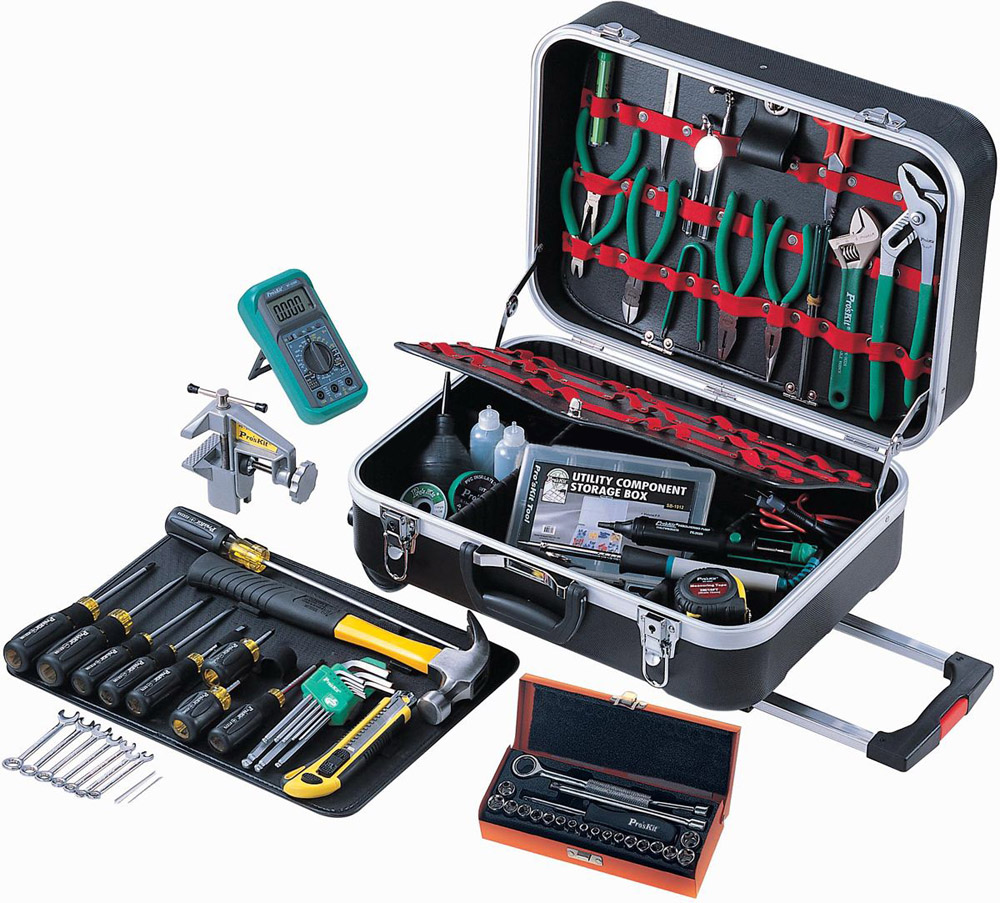
\includegraphics[height=0.95\textheight]{tech/tools/proskit/PK5308BM.jpg}

\textbf{PK-5308BM универсальный набор инструментов}

\clearpage
\noindent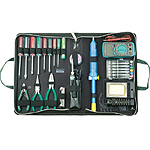
\includegraphics[height=0.95\textheight]{tech/tools/proskit/1PK-616B.jpg}

\textbf{1PK-616B Набор инструментов для электроники профессиональный}

\clearpage\label{1PK-813B}
\noindent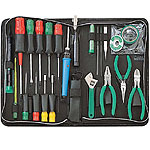
\includegraphics[height=0.95\textheight]{tech/tools/proskit/1PK-813B.jpg}

\textbf{1PK-813B Набор базовых инструментов для электроники}

\clearpage

По личному опыту: в 1PK-813B не хватает

\begin{itemize}
  \item мелкого мультиметра,
  \item стриппера 1PK-3001E,
  \item микрокусачек типа 8PK-30D,
  \item канифоли,
  \item ножа,
  \item настроечную отвертку заменить индикаторной.
\end{itemize}

\clearpage
\secrel{Инструмент до 1000\,В}

Для электромонтажных работ обязательно приобретите комплект
высоковольтного инструмента до 1000\,В:

\begin{tabular}{p{0.45\textwidth} p{0.45\textwidth}}
\noindent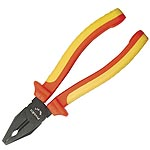
\includegraphics[width=0.45\textwidth]{tech/tools/proskit/PM-911.jpg}
&
\noindent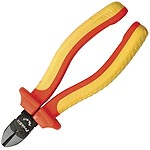
\includegraphics[width=0.35\textwidth]{tech/tools/proskit/PM-917.jpg}
\\

\textbf{PM-911 Пассатижи 1\,кВ}
&
\textbf{PM-917 Кусачки (бокорезы) 1\,кВ}
\\
\end{tabular}
\clearpage

\secrel{Хранение}

\begin{tabular}{p{0.45\textwidth} p{0.45\textwidth}}
\noindent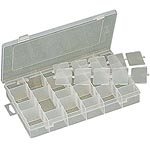
\includegraphics[width=0.45\textwidth]{tech/tools/proskit/103-132D.jpg}
&
\noindent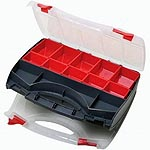
\includegraphics[width=0.45\textwidth]{tech/tools/proskit/SB-3428SB.jpg}
\\
\textbf{103-132D Кассетница для деталей и компонентов}
&
\textbf{SB-3428SB Портативная кассетница для саморезов и т.п.}
\\
\end{tabular}
\clearpage

\secrel{Радиомонтаж}

\begin{tabular}{p{0.45\textwidth} p{0.45\textwidth}}
\noindent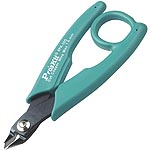
\includegraphics[width=0.45\textwidth]{tech/tools/proskit/8PK-30D.jpg}
&
\noindent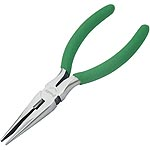
\includegraphics[width=0.45\textwidth]{tech/tools/proskit/1PK-709.jpg}
\\
\textbf{8PK-30D Кусачки миниатюрные}
&
\textbf{1PK-709 Длинногубцы-кусачки}
\\
\end{tabular}
\clearpage

\begin{tabular}{p{0.45\textwidth} p{0.45\textwidth}}
\noindent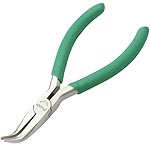
\includegraphics[width=0.45\textwidth]{tech/tools/proskit/1PK-055S.jpg}
&
\noindent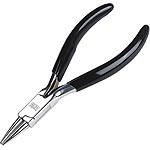
\includegraphics[width=0.45\textwidth]{tech/tools/proskit/1PK-29.jpg}
\\
\textbf{1PK-055S Длинногубцы изогнутые}
&
\textbf{1PK-29 Круглогубцы}
\\
\end{tabular}
\clearpage

\begin{tabular}{p{0.45\textwidth} p{0.45\textwidth}}
\noindent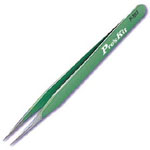
\includegraphics[width=0.45\textwidth]{tech/tools/proskit/1PK-101T.jpg}
&
\noindent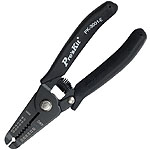
\includegraphics[width=0.45\textwidth]{tech/tools/proskit/1PK-3001E.jpg}
\\
\textbf{1PK-101T Пинцет прямой}
&
\textbf{1PK-3001E Клещи для зачистки проводов прецизионные (стриппер)}
\\
\end{tabular}
\clearpage

\begin{tabular}{p{0.45\textwidth} p{0.45\textwidth}}
\noindent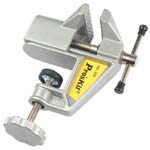
\includegraphics[width=0.45\textwidth]{tech/tools/proskit/PD-374.jpg}
&\\
\textbf{PD-374 Тиски на струбцине}
&\\
\end{tabular}
\clearpage

\secrel{Прочие}

Попалась интересная недорогая отвертка: aиксация четкая, исполнение очень
неплохое, позволяет добраться до узких мест. Из минусов: ручка похоже не
цельнометаллическая, при изломе есть риск распороть руку.

\bigskip
\noindent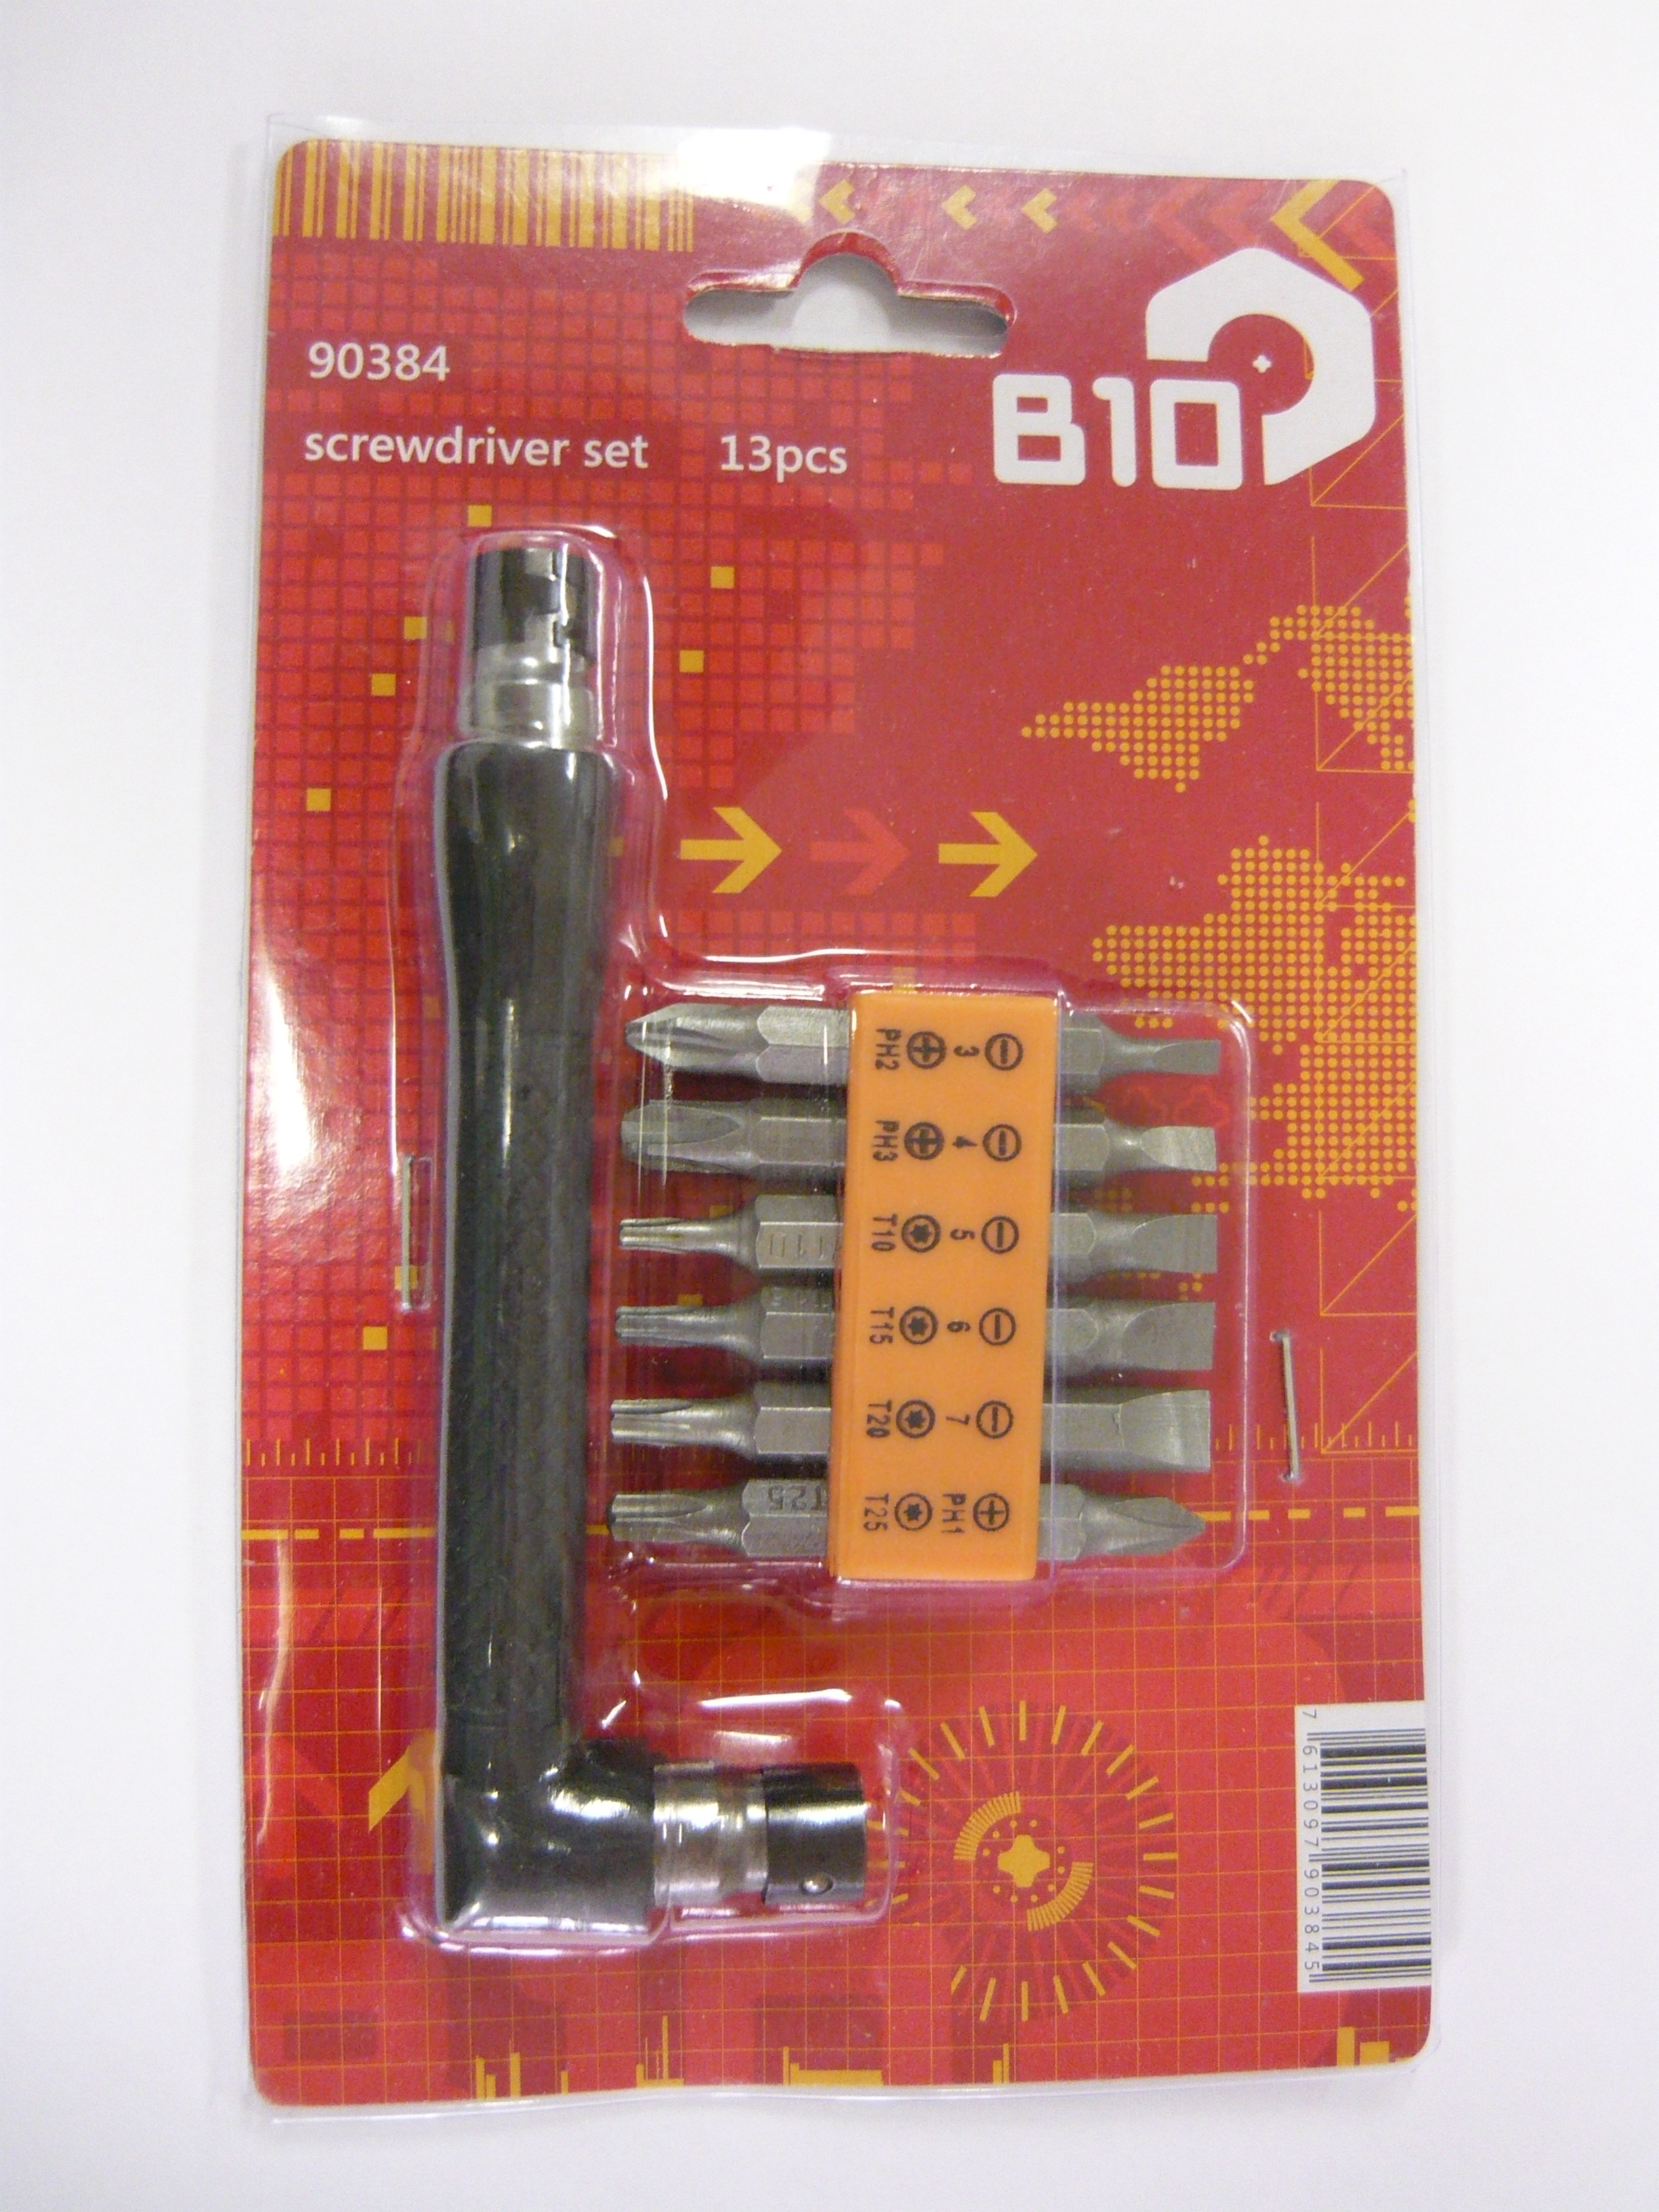
\includegraphics[width=0.4\textwidth]{tech/tools/P1020966.jpg}
\noindent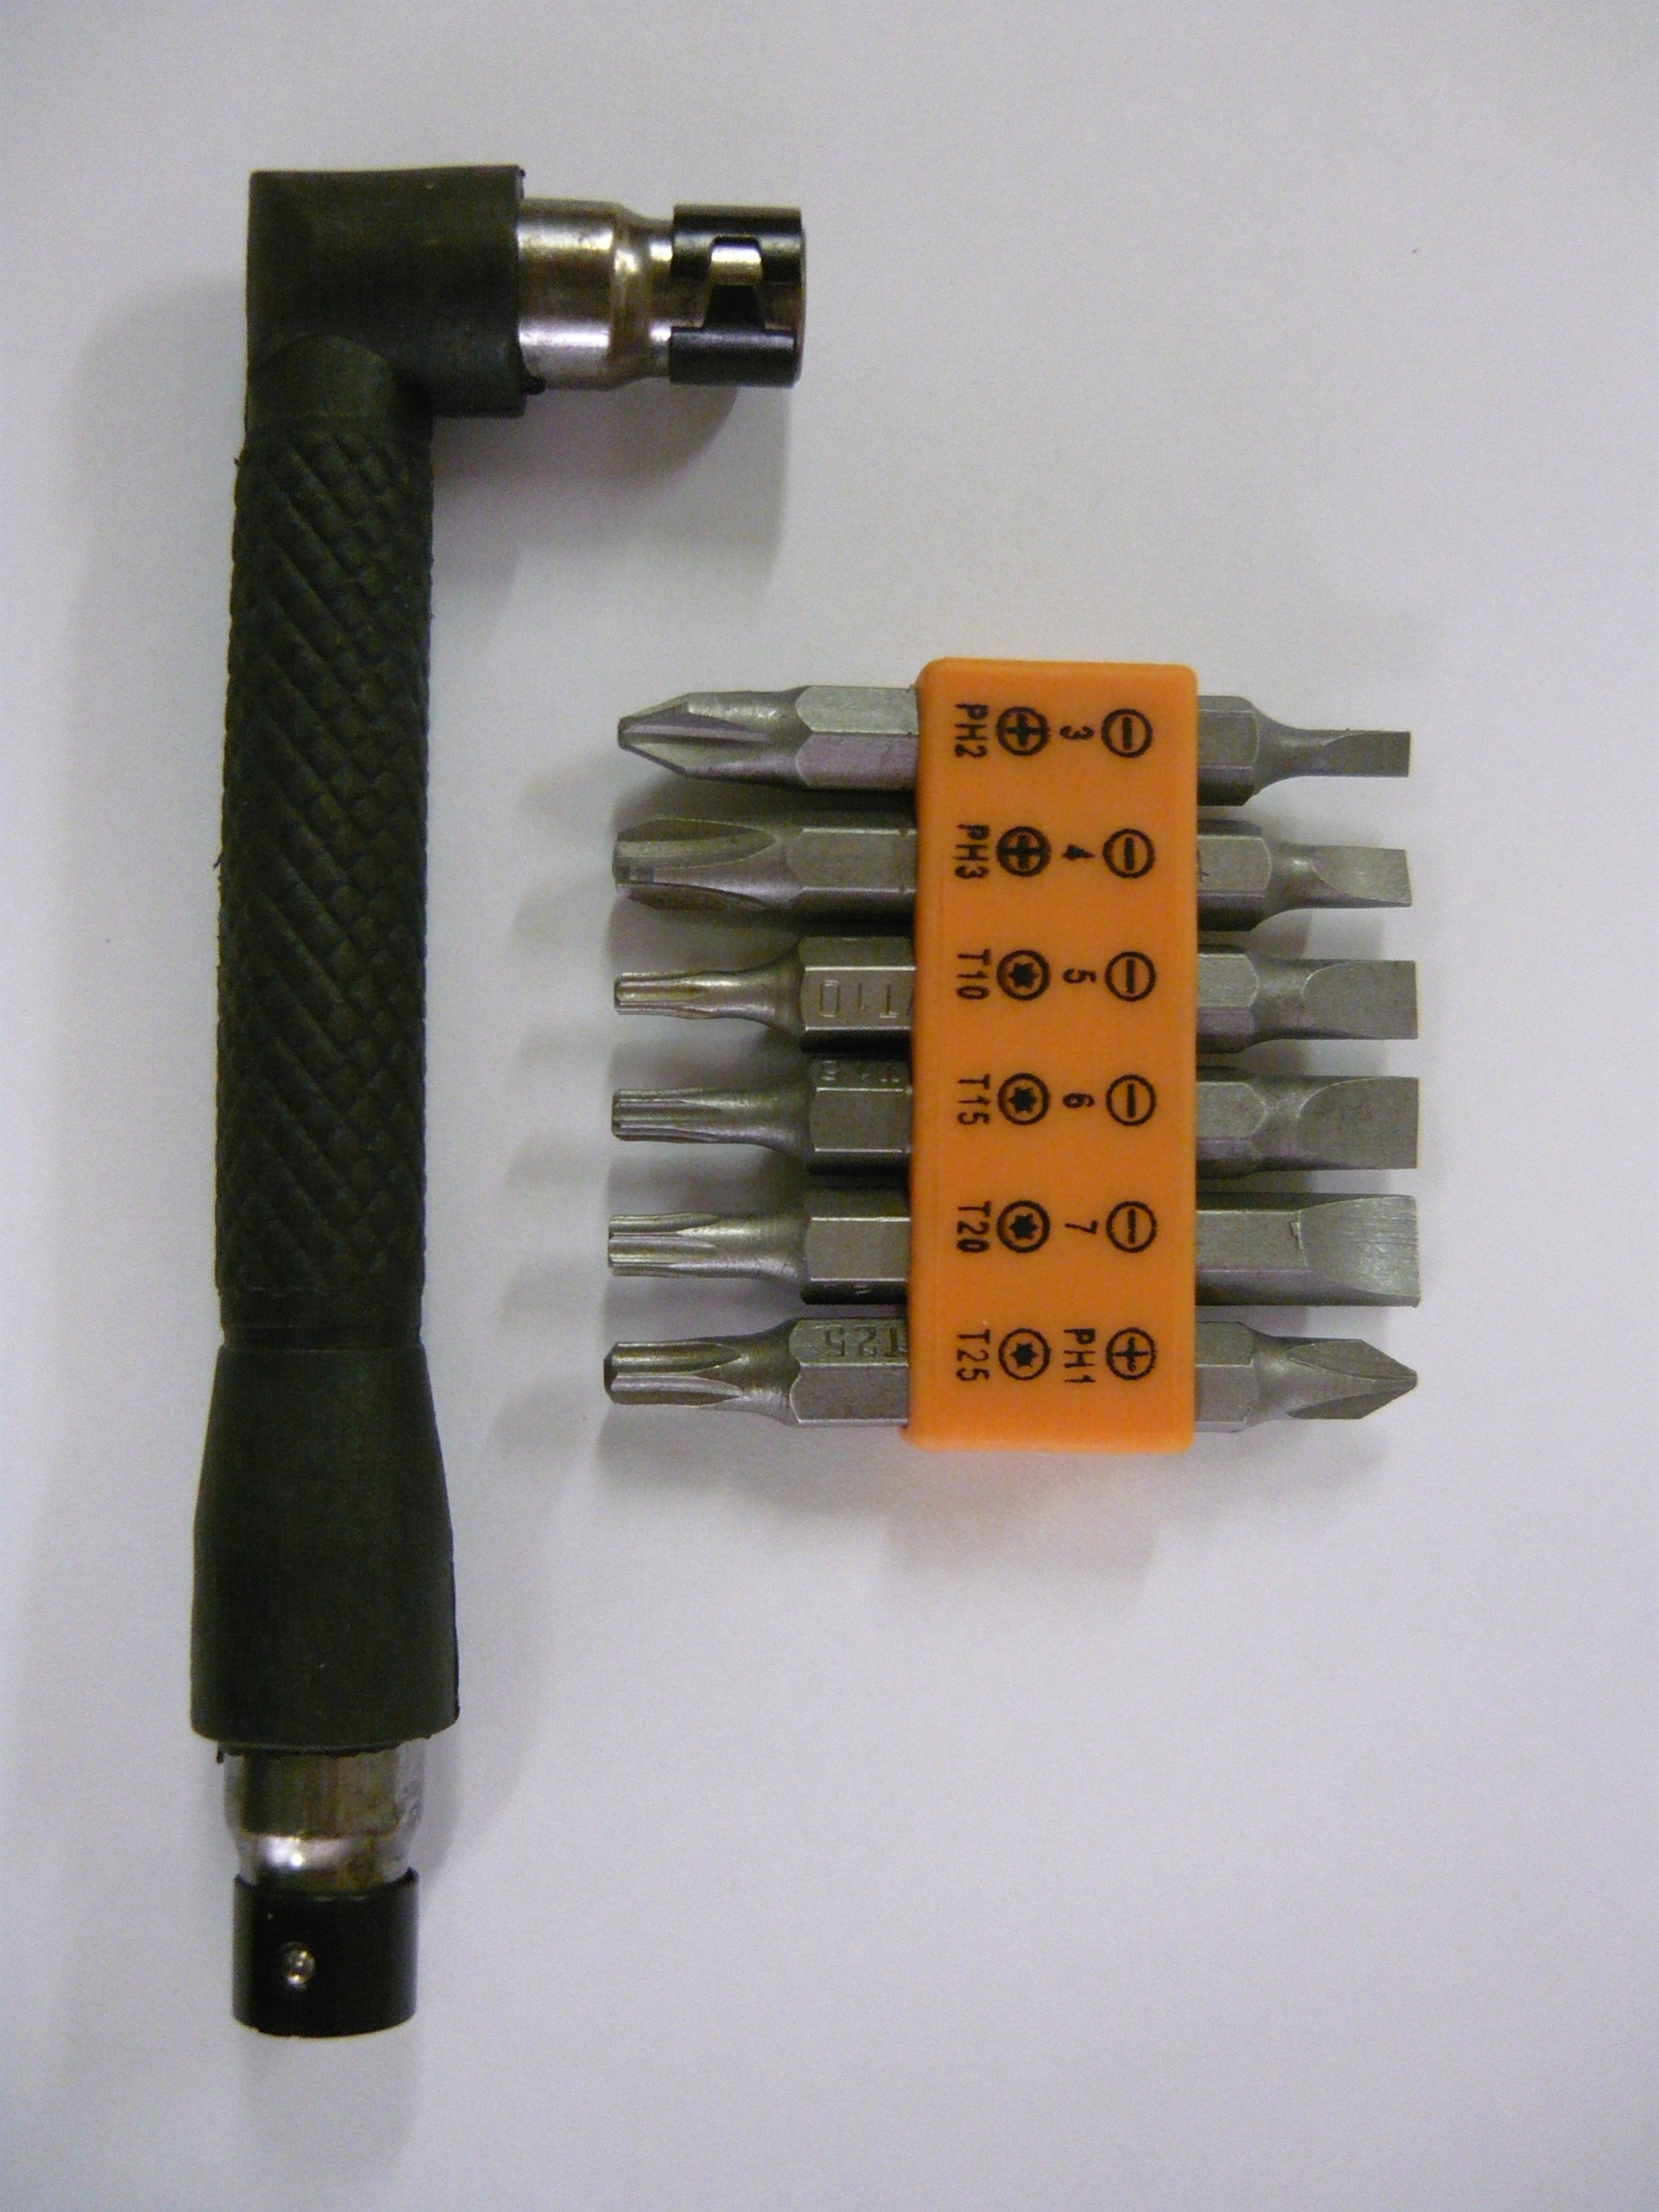
\includegraphics[width=0.4\textwidth]{tech/tools/P1020967.jpg}
\clearpage

\secup




\section{Паяльное оборудование}

\subsection{Паяльник}

Паяльник\ --- обязателен дешевый сетевой мощностью не менее 20\,Вт, типа
ЭПСН-25/220. Ограничитель мощности или регулятор температуры легко собрать
самостоятельно.

Для сборки электроники хорошо также иметь маленький монтажный 12\,В 8\,Вт от
паяльной станции ZD-927 ($\sim$100\,р), без самой станции. Если не жалко 500\,р,
берите станцию ZD-927 целиком, внутри простейший регулятор мощности, и вам не
понадобится источник питания на 12\,В, который вы еще не сделали.

\noindent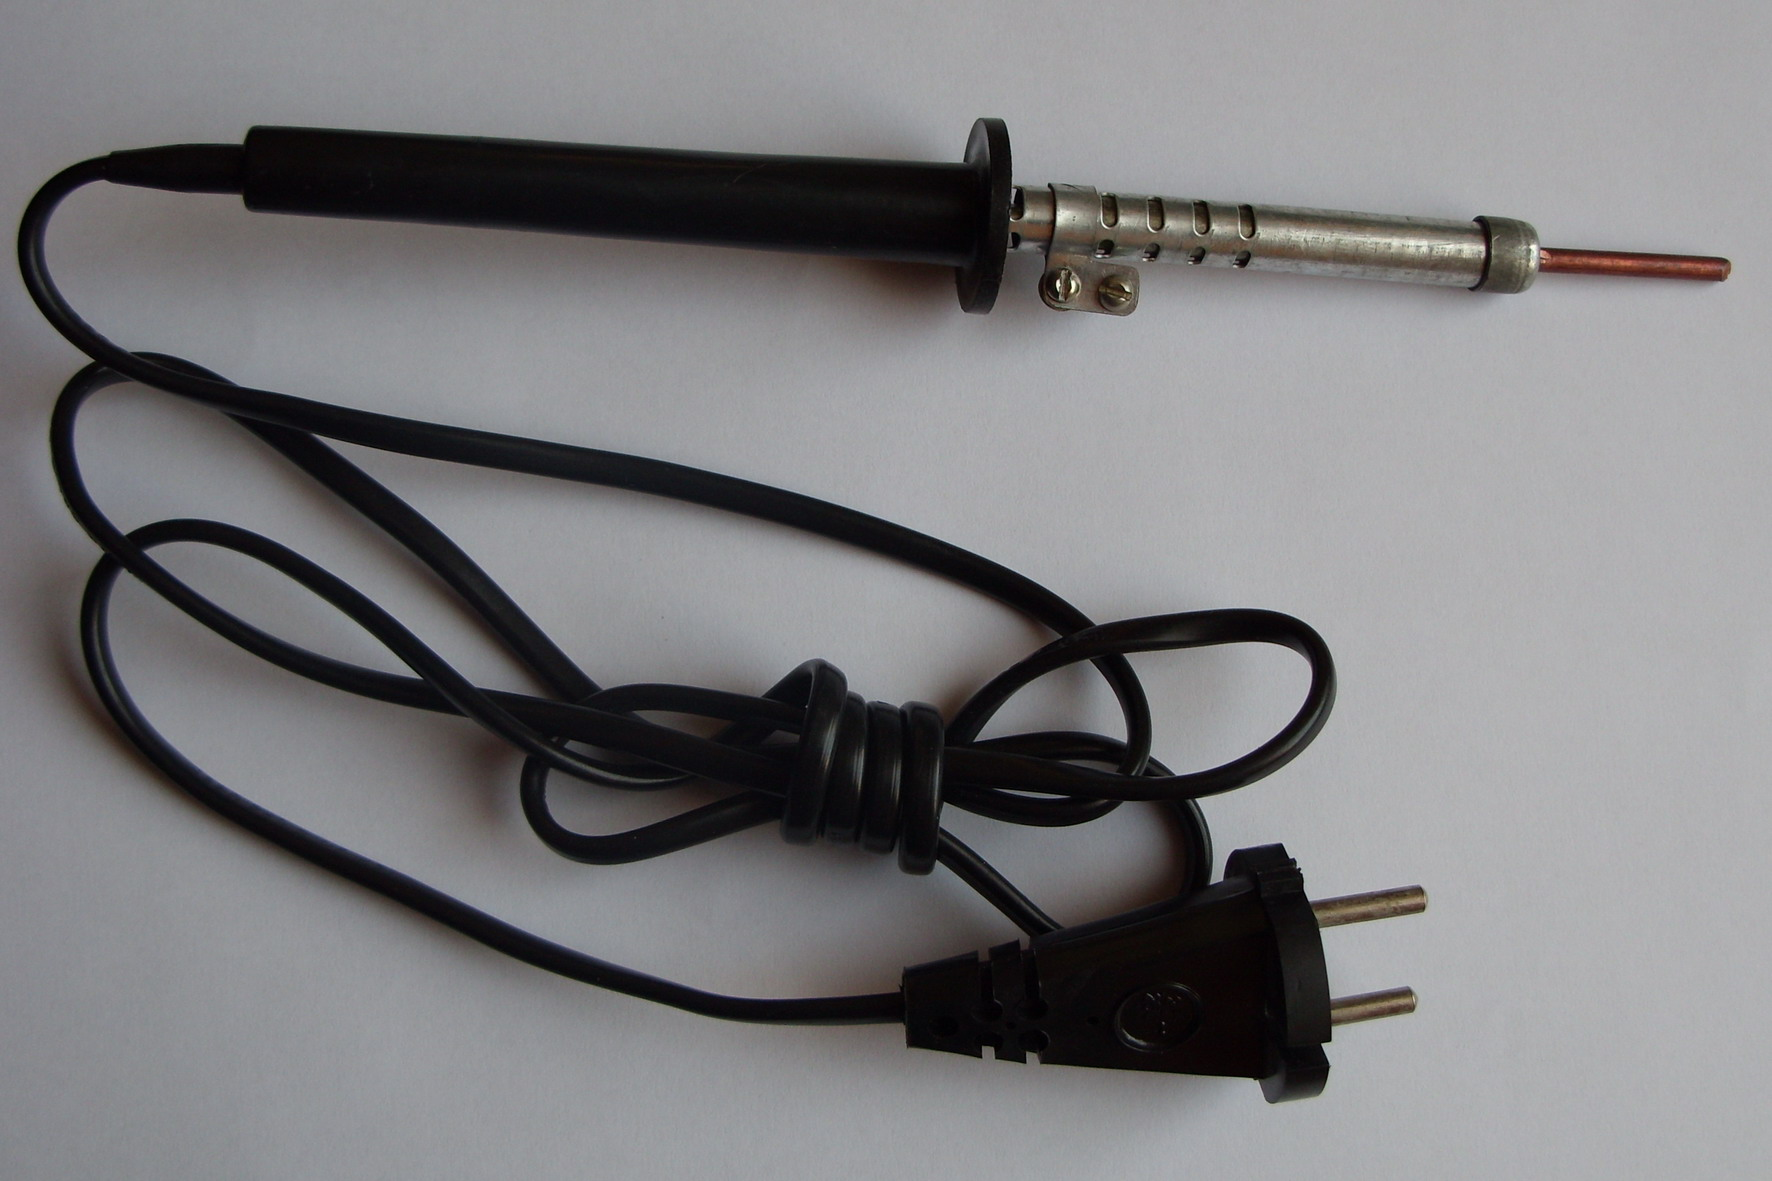
\includegraphics[width=0.4\textwidth]{tech/tools/solder/EPSN25.jpg}
\textbf{Паяльник ЭПСН-25/220}

\noindent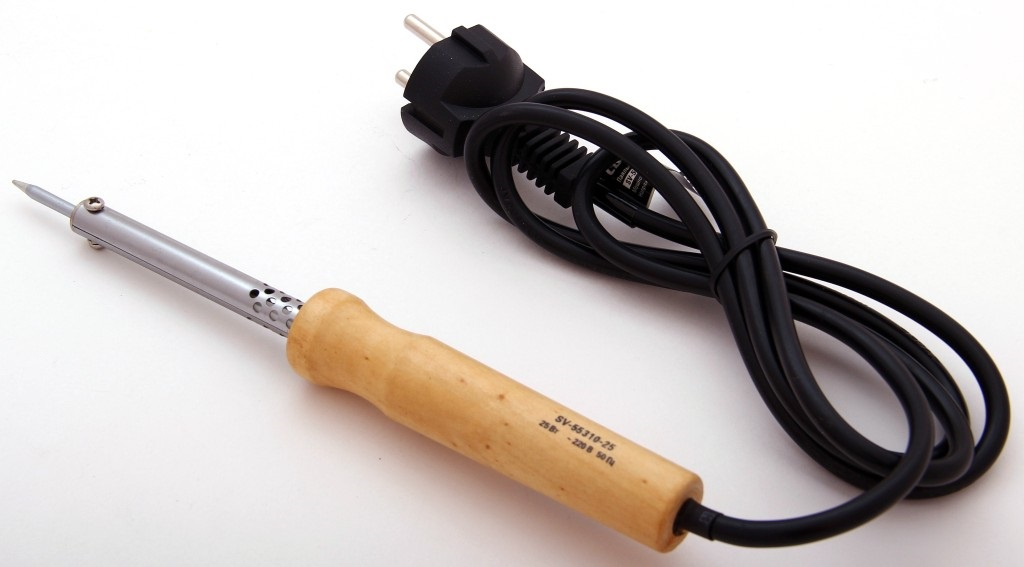
\includegraphics[width=0.4\textwidth]{tech/tools/solder/SV-55310-25.jpg}
\textbf{Паяльник 220В 25Вт, СВЕТОЗАР, SV-55310-25 230\,р.}

\noindent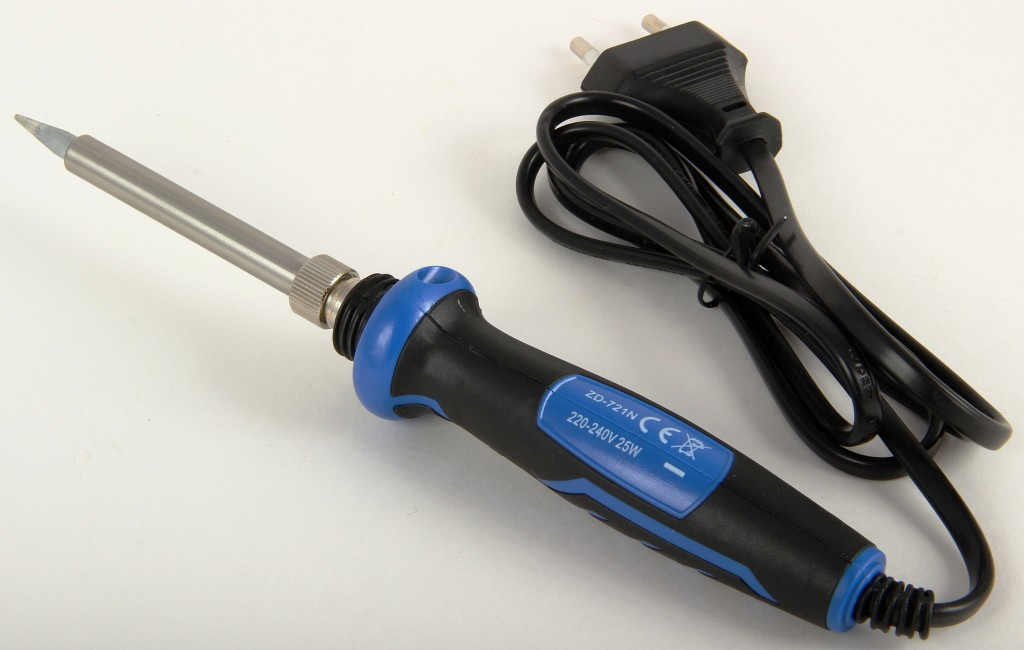
\includegraphics[width=0.4\textwidth]{tech/tools/solder/ZD-721N.jpg}
\textbf{Паяльник 220В 25Вт ZD-721N 175\,р.}

\noindent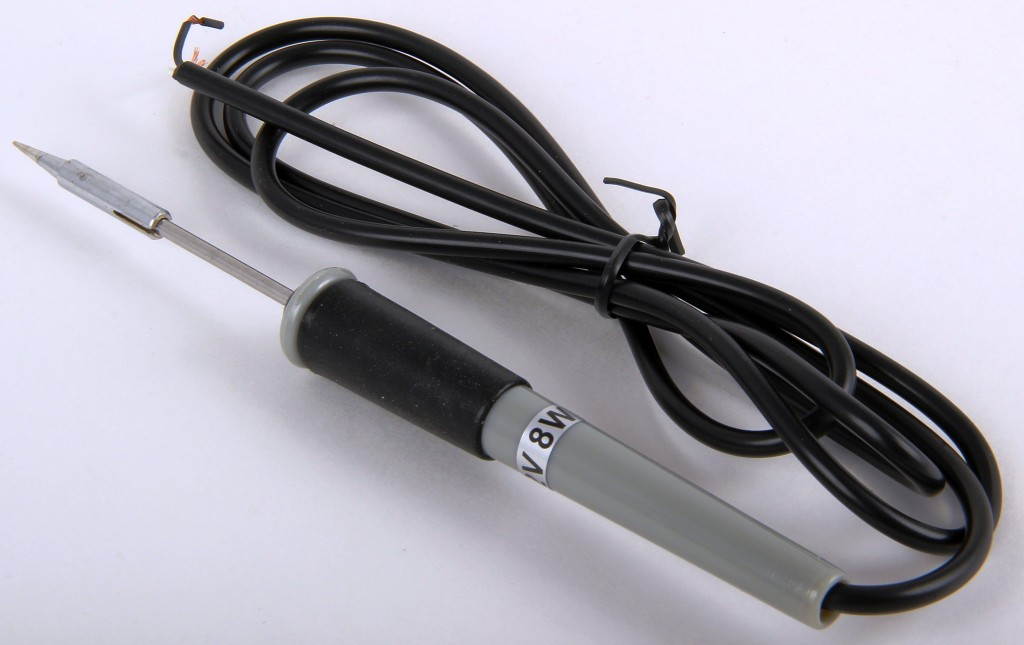
\includegraphics[width=0.4\textwidth]{tech/tools/solder/Iron8W.jpg}
\textbf{Паяльник для станции ZD-927 12\,В 8\,Вт 85\,р.}

\subsection{Паяльная станция}

Из всего разнообразия для хоббита оптимальным являются паяльные станции Lukey
702/853D (3000+\,р). Для работы или регулярного хобби паяльная станция с феном,
а может даже и встроенным источником питания, вещь незаменимая, и не такая уж
дорогая.

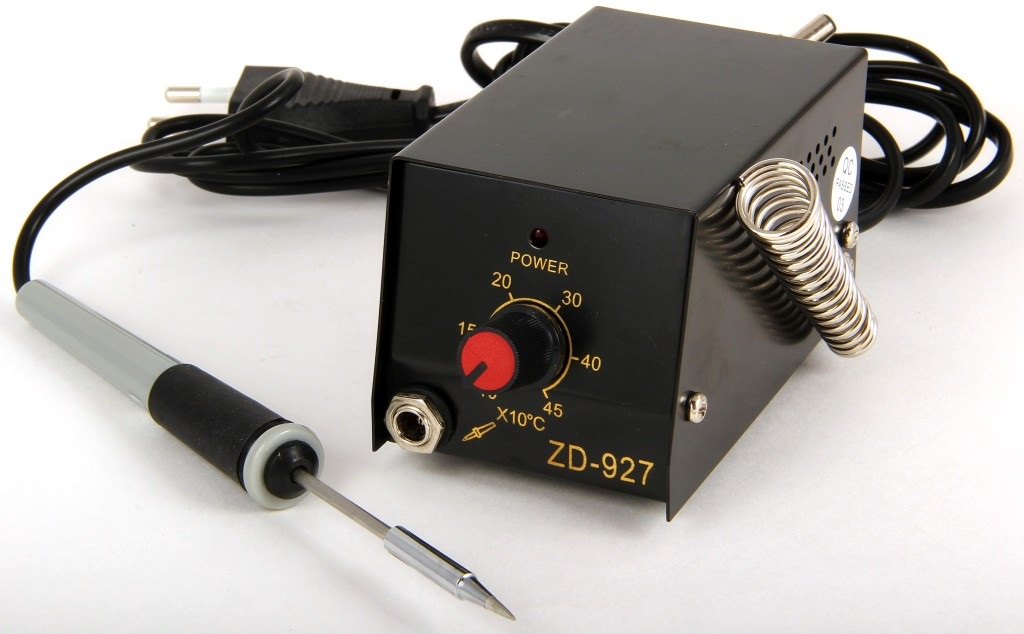
\includegraphics[width=0.45\textwidth]{tech/tools/solder/ZD927.jpg}
\textbf{Паяльная станция ZD-927 520\,р.}

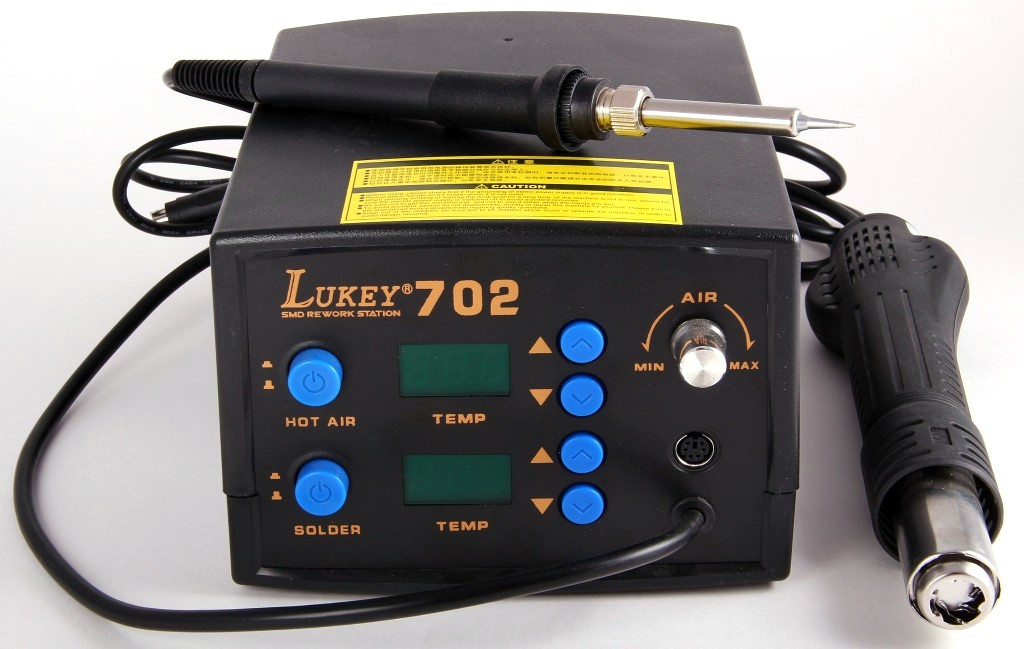
\includegraphics[width=0.45\textwidth]{tech/tools/solder/Lukey702.jpg}
\textbf{Паяльная станция LUKEY 702 3100\,р.}

\clearpage
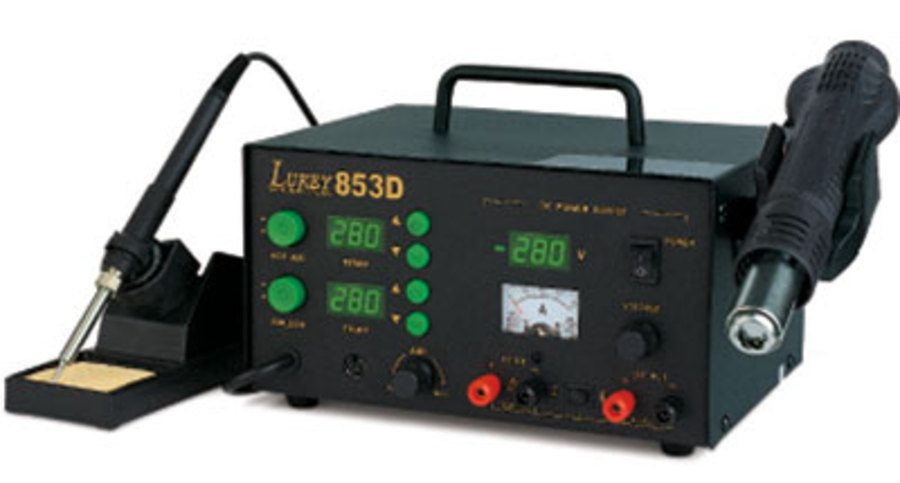
\includegraphics[width=0.95\textwidth]{tech/tools/solder/Lukey853D.jpg}

\textbf{Паяльная станция LUKEY 853D с источником питания 5200\,р.}
\clearpage



% \section{JTAG-адаптер}
% 
% % \input{jtag/soft}
% % \input{stlink/stlink1}
% 
% \section{Отладочные платы}
% 
% Прежде чем начать работать с отдельными \mk, устанавливая их на плату
% собственной разработки, для быстрого старта используют \term{отладочные
% платы}\note{development board, demo board}
% 
% \subsection{Arduino /Atmel Mega AVR8/}
% 
% \subsection{Cortex-Mx} %См. \ref{devkitcmx}
% 
% \subsection{CubieBoard /Cortex-A8 AllWinner A10/}
% 
% \subsection{Raspberry Pi /ARM11 BCM3032/}
% 
% \subsection{BlackSwift /MIPS/}
% 
% \subsection{VoCore /MIPS/}

\secrel{Измерительное оборудование}\secdown

\secrel{Мультиметр}\label{mmetr}

\emph{Мультиметр\ --- обязателен, без него работать невозможно}\note{или
собирать замену на паре измерительных головок тока/напряжения, и делителях}.
Для совсем начинающего больше всего подойдет M320\ref{mmetr320} c
автодиапазоном, когда освоитесь возьмете вторым прибором что-то из крупных серий
M89x/MY6x с измерением температуры\note{иногда нужно для измерения температуры
корпусов элементов, радиаторов, растворов если возитесь с электрохимией}
или ``рыльцеметр''\ref{rlcmetr} (RLC).

\secdown
\secrel{Mastech M838}\label{mmetr838}

\begin{tabular}{p{0.3\textwidth} p{0.6\textwidth}}
\noindent\includegraphics[width=0.3\textwidth]{tech/tools/mes/M838.jpg}
&
Простой, компактный, дешевый, \emph{с измерением температуры}
\\
\end{tabular}

\secrel{Mastech M300}\label{mmetr300}

\begin{tabular}{p{0.3\textwidth} p{0.6\textwidth}}
\noindent\includegraphics[width=0.3\textwidth]{tech/tools/mes/M300.jpg}
&
Простой, \emph{очень компактный}, дешевый, в чехле очень удачно умещается в
набор инструментов.
\\
\end{tabular}

\secrel{Mastech M320}\label{mmetr320}

\begin{tabular}{p{0.3\textwidth} p{0.6\textwidth}}
\noindent\includegraphics[width=0.3\textwidth]{tech/tools/mes/M320.jpg}
&
То же что и M300\ref{mmetr300}, но с \emph{автодиапазоном}, т.е. не требует
переключения диапзонов измерения вручную. На любителя, возможно \emph{удобен для
совсем начинающих}, но слишком медленен если требуется измерение меняющегося
тока/напряжения.
\\
\end{tabular}

\secup

\secrel{Осциллограф}

\secrel{Логический анализатор}

\secrel{Генератор сигналов}

\secrel{Рыльцеметр RLC}\label{rlcmetr}

\secup

\secrel{Электроинструмент}\secdown

\secrel{Дрелъ}

% \noindent
% \begin{tabular}{p{0.5\textwidth} p{0.5\textwidth}}
% \noindent
% \includegraphics[width=0.45\textwidth]{tech/tools/PraktylR.jpg}
% &
% \noindent
% \includegraphics[width=0.45\textwidth]{tech/tools/D_11_530ER.jpg}
% \\
% \textbf{Дрель ударная сетевая} & \textbf{Дрель безударная сетевая} \\
% \textbf{Praktyl-R PID13D01 400\,Вт} 
% \href{http://leroymerlin.ru/catalogue/instrumenty/elektroinstrument/dreli\_udarnye/13805983/}{\textbf{(!)395\,р.}}
% &
% \textbf{Интерскол Д-11/530ЭР (с БЗП)}
% \href{http://leroymerlin.ru/catalogue/instrumenty/elektroinstrument/dreli\_bezudarnye/11857763/}{\textbf{1120\,р.}}
% \\
% \end{tabular}
% \bigskip
% 
% Дрель\ --- одноразовая китайчатина от 400\,р. Продаются уже брендированные на
% Леруа Мерлен, наклейка <<PID13D01 Ударная дрель 400\,Вт, 13\,мм>>. Скорость
% регулируется глубиной нажатия курка, крутилка на курке ограничивает глубину
% механически, фиксатор держит скорость близко к минимальной, запаха горелой
% пластмассы через несколько минут работы на холостом ходу нет.
% 
% По надежности рекомедуется Интерскол 1100+\,р. Надежность Интерскола\ --- не
% <<китай>>, классика ДУ-580ЭР работает в хвост и гриву, используется криворукими
% студентами, лежит в подвале в пыли от точила, и никаких вопросов даже со
% щетками.
% 
% Если не планируете много сверлить бетон, \textbf{берите дрель без ударного
% механизма}: отсутствуют лишние продольные перемещения, что может быть важно при
% использовании в качестве шпинделя сверлильного станка, и механизации других
% технологических поделок.
% 
% У шуруповерта нет 43\,мм шейки для фиксации, поэтому как средство электропривода
% он практически бесполезен, и нужен собственно для заворачивания большого
% количества саморезов. Хотя наличие ограничителя крутящего момента и малые
% габариты удобны при сверлении и сборке поделок.
% 
% \bigskip
% Имея некоторое количество поделочного материала, кривые руки и особенно доступ к
% станочному оборудованию, можно сколкозить некоторое подобие настольных
% станочков\ \pref{fig:drelstans}\ для механизации некоторых работ,
% используя дрель в качестве привода.
% 
% Главным элементом такой оснастки\ --- зажим на шейку дрели 43\,мм. Особых
% требований по его точности и качеству нет, т.к. сама шейка обычно пластиковая, и
% никакой доводки по круглости и параллельности оси инструмента не проходит.
% 
% \clearpage
% \phantomsection\label{fig:drelstans}
% \noindent\includegraphics[height=0.528\textheight]{tech/tools/DrelLathe.jpg}
% \noindent\includegraphics[height=0.528\textheight]{tech/tools/DrelShliph.jpg}
% 
% \noindent\includegraphics[height=0.465\textheight]{tech/tools/DrelLathe2.jpg}
% \noindent\includegraphics[height=0.465\textheight]{tech/tools/DrelBoren.jpg}
% \clearpage

\secrel{Лобзик}

% \noindent
% \begin{tabular}{p{0.5\textwidth} p{0.5\textwidth}}
% \noindent
% \includegraphics[width=0.45\textwidth]{tech/tools/LobzPraktyl.jpg}
% &
% \noindent
% \includegraphics[width=0.45\textwidth]{tech/tools/LobzMakita4329.jpg}
% \\
% \href{http://leroymerlin.ru/catalogue/instrumenty/elektroinstrument/lobziki/13805991/}{\textbf{Praktyl
% 350 Вт 356\,р.}} 
% & 
% \href{http://leroymerlin.ru/catalogue/instrumenty/elektroinstrument/lobziki/12114283/}{\textbf{Makita
% 4329 2260\,р.}}
% \\
% \end{tabular}
% \bigskip
% 
% Лобзик полезен при разделке стеклотекстолита, и изготовлении технологической
% мебели (стеллажи, рабочие столы и т.п.).

\secrel{Жвигатель}

% Если у вас возникло желание механизировать изготовление механических деталей, а
% свободного доступа к настоящему станочному оборудованию нет, есть смысл
% рассмотреть изготовление самодельной механизированной оснастки 
% типа\ \pref{fig:drelstans}, или даже самодельных станочков. В этом случае надо
% рассмотреть применения универсального привода.
% 
% Первый кандидат на место универсального электропривода достается той самой
% дрели, не забываем об обязательном наличии 43\,мм монтажной шейки.
% Достоинство дрели как привода\ --- прямое подключение к сети, встроенный
% редуктор, есть модели с простой регулировкой оборотов, есть резьба и отверстие
% под винт на валу, в комплекте есть патрон для зажима мелких деталей в
% точилке\footnote{\ БЗП удобен, патрон с ключем дает лучший зажим и возможно
% точнее}.
% 
% Ограниченно доставаемые двигатели от стиральных машин, отличаются мощностю и
% оборотистостью, особенно от старых моделей. Часто доступны сразу с готовым
% шкивом на валу, который иногда проще использовать, чем снять.
% 
% Автозапчасти: привод печки Камаза, двигатель постоянного тока 
% 24\,В 50\,Вт
% 
% Новые асинхронные двигатели АИРЕ 56 B2/B4 (3000/1500 об.) с заводским
% конденсатором, подключается к сети $\sim$220\,В, цена от 2500\,р.
% С ростом размеров и мощности цена резко повышается.
% Следует обратить внимание на возможность монтажа на дополнительный фланцевый
% подшипниковый щит, (?) с моделями АИРЕ 80.
% 
% Для самодельных серлилок и микроинструмента хороши китайские воздушные шпиндели
% постоянного тока с цанговыми патронами ER11. Требуют источник питания
% постоянного тока 9$\div$48\,В. В магазинах не попадались, необходима прямая
% покупка с \href{http://www.aliexpress.com/}{AliExpress}\note{пользуйтесь
% английской версией\ --- переводная жуткое УГ}\ по почте.
% 
% % \clearpage
% \begin{tabular}{l l}
% 
% \noindent\includegraphics[width=0.37\textwidth]{tech/tools/VyatkaDvig.jpg} 
% & 
% \noindent\includegraphics[width=0.37\textwidth]{tech/tools/KamazDvig.jpg}
% \\
% \textbf{Жвигатель Вятка-Автомат 19??\,г.}
% &
% \textbf{Двигатель печки Камаза}
% \\
% 
% \noindent\includegraphics[width=0.37\textwidth]{tech/tools/AIRE.jpg}
% & 
% \noindent\includegraphics[width=0.37\textwidth]{tech/tools/ER11.jpg}
% \\
% \textbf{АИРЕ 56 B2, 0.2\,КВт}
% &
% \textbf{Воздушный шпиндель с цангой ER11}
% \\
% 
% \end{tabular}
% \clearpage
% 
% Съемные фрезерные шпиндели, поставляются отдельно или в комплекте с насадкой
% ручного фрезера по дереву. Лучшие, со стальной шейкой\ --- Kress, активно
% применяются хобби-ЧПУшниками. Попроще и сильно дешевле делал Интерскол, иногда
% попадается noname. Недостаток как универсального привода\ --- они
% высокоскоростные, возникают проблемы с понижающими передачами. Применение\ ---
% приводной высокоскоростной инструмент: боры, фрезы по дереву, микроинструмент
% для граверов (микродиски, шарошки). Цанга 8\,мм. Для некоторых моделей бывают
% наборы цанг на мелкий инструмент.
% 
% \bigskip
% \begin{tabular}{p{0.3\textwidth} p{0.3\textwidth} p{0.3\textwidth} }
% \noindent\includegraphics[height=0.3\textheight,width=0.3\textwidth,keepaspectratio]{tech/tools/Kress530.jpg}
% &
% \noindent\includegraphics[height=0.3\textheight,width=0.3\textwidth,keepaspectratio]{tech/tools/Interskol30.jpg}
% &
% \noindent\includegraphics[height=0.3\textheight,width=0.3\textwidth,keepaspectratio]{tech/tools/InterskolFM55.jpg}
% \\
% KRESS 530/800/1050 FM(E)
% &
% Интерскол ФМ-30/750
% &
% Интерскол ФМ-55/1000 Э
% \\
% \href{http://kress-shop.ru/product/frezernyj-dvigatel-530-fm-kress-06082302/}{5600+\,р.}
% &
% /снят с производства/
% &
% \href{http://www.kuvalda.ru/catalog/1867/27920/}{5050\,р.}
% \\
% \end{tabular}

\secup



\secup


\chapter{Трассировка плат и подготовка производства в KiCAD}

\section{Технология ЛУТ (Лазерный УТюг)}

\section{Технология фоторезиста}

\section{Формат Gerber и подготвка промышленного производства}


\chapter{FreeCAD}

\section{Чертеж}

\section{Эскиз}

\section{Деталь}

\section{Сборка}

\section{Автогенерация конструкторской докуметации}

\section{Скрипты и пользовательские расширения}



\chapter{Эксплуатация станочного оборудования}

\chapter{Основы ЧПУ и цифрового производства}

\section{CAM-пакеты для FreeCAD}

\part{Основы теории систем автоматического управления}

\chapter{Математический аппарат}

\section{Передаточная функция}

\section{Устойчивость САУ}

\section{Сети Петри}

\section{Автоматы Маркова}

\chapter{Релейное управление}

\chapter{Пропорциональные САУ}

\chapter{ПИДn-регуляторы}

\part{Разработка ПО для встраиваемых систем}

\chapter{Вспомогательные скрипты на языке \py}

\begin{tabular}{p{0.1\textwidth} p{0.8\textwidth}}
\includegraphics[width=0.1\textwidth]{python/logo.png}&
\emph{
Название языка произошло вовсе не от вида пресмыкающихся. Автор назвал язык в
честь популярного британского комедийного телешоу 1970-х «Летающий цирк Монти
Пайтона». Впрочем, всё равно название языка чаще ассоциируют именно со змеёй,
нежели с передачей\ --- пиктограммы файлов в KDE или в Microsoft Windows и даже
эмблема на сайте \url{http://www.python.org} (до выхода версии 2.5) изображают
змеиные головы.
}
\\
\end{tabular}
\bigskip

\py\note{в оригинале читается \textbf{п\'{а}йтон}, но давно русифицировался как
\textbf{пит\'{о}н}}\ --- высокоуровневый язык программирования общего
назначения, ориентированный на повышение производительности разработчика и
читаемости кода.

\py\ удобно применять для написания различных вспомогательных скриптов.
Часто его используют при разработке сложных программных систем для написания
первых версий. В процессе работы над большими программами часто перерабатываются
большие объемы кода, поэтому для ускорения разработки требуется максимально
высокоуровневый язык. После того как архитектура программы стабилизируется,
узким местом становится производительность, и программу переписывают на более
низкоуровневом компилируемом языке, чаще всего \cpp.

Написание программ упрощают:

\begin{itemize}
  \item \textbf{объектно-ориентированное программирование} облегчает разработку
  программ, позволяет переопределить стандартные операторы для пользовательских
  типов данных, упрощая синтаксис
  \item \textbf{динамическая типизация} не требуется заранее упределять
  переменные, они создаются простым присваиванием
  \item \textbf{обработка исключений} для секции кода можно определить
  обработчик ошибок
  \item \textbf{высокоуровневые структуры данных}\ --- списки, словари (набор
  элементов ключ:значение), очереди
  \item богатая стандартная библиотека и множество дополнительных библиотек на
  все случаи
\end{itemize}

\section{Установка под \win}\label{pywinstall}

\bigskip
\menu{
\keys{\winstart+R}
>
\url{http://www.python.org}
>
Downloads
>
\href{https://www.python.org/ftp/python/2.7.8/python-2.7.8.msi}{Python 2.7.8}
}

\bigskip
\menu{\file{python-2.7.8.msi}
>
Setup>
for all users/for me
}

\menu{Destination Directory > \file{C:/Python/} > Next}

\nopagebreak
\bigskip
\includegraphics[width=0.45\textwidth]{python/install/037.png}
\includegraphics[width=0.45\textwidth]{python/install/038.png}
\bigskip


\menu{Customize > Python > Add python.exe to PATH > Next > Finish}

\nopagebreak
\bigskip
\includegraphics[width=0.45\textwidth]{python/install/039.png}
\includegraphics[width=0.45\textwidth]{python/install/045.png}
\bigskip

\section{Дополнительные материалы}

\cite{pyotkidach} Г. Россум, Ф.Л.Дж. Дрейк, Д.С. Откидач, 
\href{http://rus-linux.net/MyLDP/BOOKS/python.pdf}{Язык программирования Python}

\cite{pythink} Аллен Дауни
\href{https://drive.google.com/file/d/0B0u4WeMjO894Q2hWV1QwOFFQOVk/view?usp=sharing}{Думать
на языке \py: Думать как компьютерный специалист}



\chapter{Make: управление сборкой проектов}\label{make}

\chapter{VCS: cистемы контроля версий}\label{vcs}

\section{CVS}

\section{Subversion}

\section{Git}

\subsection{GitHub}

\chapter{Основы Си и \cpp}

\subsection{Установка MinGW (win32)}

\section{Особенности \cpp\ в embedded}

\chapter{LLVM и разработка собственных компиляторов}

\section{Лексический и синтаксический анализ}

\section{Применение flex/bison для разбора текстовых форматов данных}

\section{Компилятор Паскаля}

\chapter{Сборка кросс-компилятора GNU toolchain}

\part{Микроконтроллеры \cmx}

\chapter{Отладочные платы}\label{devkitcmx}

\section{STM32DISCOVERY /Cortex-M3 STM32F103/}

\section{STM32F4DISCOVERY /Cortex-M4 STM32F407/}



\part{Периферия}

\part{Встраиваемый \emlinux}

\chapter{cross}

\chapter{BuildRoot}

\chapter{Особенности OpenWrt}

\chapter{Библиотека SDL}

\section{Реализация microGUI}

\chapter{Приложения для X Window}

\chapter{Программирование сетевых приложений}

\chapter{Сборка кросс-компиляторя GNU мальтийским крестом}

\part{IDE}

IDE\ --- Integrated Development Environment, интегрированная среда разработки.

Программный пакет, включающий 
\begin{itemize}
  \item средства управления проектом,
  \item отслеживание зависимостей между файлами (в т.ч. с анализом исходного
  текста программ на конструкции типа \verb|#include|, \verb|module|,
  \verb|uses|),
  \item автозапуском компиляторов для изменившихся файлов,
  \item GUI для отладчиков (gdb),
  \item специализированный редактор plain text\note{файлы не включающие
  непечатаемых символов и бинарных данных, которые можно причитать простым
  выводом на экран командами типа \textbf{type}, \textbf{cat}, \textbf{more}}
  файлов c
  \begin{itemize}
    \item цветовой и шрифтовой \term{подстветкой синтаксиса},
  	\item \term{автодополнением}: дописываются имена объектов программ, 
  	синтаксические конструкции и параметры функций,
 \item \term{автоформатированием}: фрагмент текста переформатируется в
 соответствии с синтаксисом языка редактируемого файла, проставляются отступы в
 зависимости от вложенности синтаксических конструкций типа циклов и условных
 блоков)
  	\item выделением строк, на которые указывают сообщения об ошибках
  	компиляторов,
  	\item маркеры точек останова отладчика
  \end{itemize}
  \item отображение структуры программ, например деревья классов и структур
  данных
  \item контекстные справочники по используемым языкам программирования,
  автоматический вывод списка параметров при вводе имени функции
  \item отображение дизассемблерных листингов для компилируемых языков
  \item отображение браузера как вкладки или MDI окна
  \item отображение вывода \term{статических анализаторов} программ c
  кликабельными ссылками
  \item вывод компиляторов и трансляторов с цветовым выделением и переход на
  ошибочную строку в редакторе при щелчке на ошибке
  \item \ldots
\end{itemize}

В этой книге рассмотрены три бесплатных мультиплатформенных OpenSource IDE, в
порядке навороченности, универсальности, и требуемым ресурсам для работы самой
среды:

\begin{enumerate}
  \item \eclipse\ \ref{eclipse}: самая навороченная и ресурсоемкая IDE, написана
  на Java, имеет десятки дополнительных модулей на все случаи, умеет работать со
  всеми распространенными языками программирования, жрет память, и требует
  современного компьютера минимум с 2+ Гб ОЗУ. Последний релиз \eclipse\ Luna
  работает заметно быстрее (особенно при запуске). 
  \item Code::Blocks \ref{cb}: легкая среда для разработки на C/\cpp, для других
  языков модет потребоваться написать свои модули или файлы описания синтаксиса
  \item \vim\ \ref{vim}: самый легкий и \emph{портабельный} универсальный
  текстовый редактор с расширенными функциями, работает на всех
  существующих платформах (кроме совсем уж embedded), использует минимум
  ресурсов, но требует некоторого обучения даже чтобы выйти из \verb|vim|
  \smiley
\end{enumerate}

\secrel{\eclipse}\label{eclipse}\secdown

\includegraphics[height=0.5\textheight]{logo/eclipse.png}

\secrel{Установка \eclipse\ под \win}

\menu{\winr>\url{https://eclipse.org/}>Download>Eclipse Luna release for>\win}

Качаем архив базовой системы:
\menu{Eclipse IDE for Java Developers>\win\ 32/64 Bit}

Или сразу сборку CDT\eclipse:
\menu{Eclipse IDE for C/C++ Developers>\win\ 32/64 Bit}

\secrel{Установка \eclipse\ под \linux}

\menu{\winr>\url{https://eclipse.org/}>Download>Eclipse Luna release for>\linux}

Качаем архив базовой системы:
\menu{Eclipse IDE for Java Developers>\linux\ 32/64 Bit}

Или сразу сборку CDT\eclipse:
\menu{Eclipse IDE for C/C++ Developers>\linux\ 32/64 Bit}

\bigskip

Пока качается, параллельно устанавливаем в систему Java-рантайм:

\begin{verbatim}
sudo aptitude install openjdk-7-jre
\end{verbatim}

Распаковывем полученный архив
\file{eclipse-java-luna-SR1-linux-gtk-x86\_64.tar.gz}
в \file{\$HOME}:

\begin{verbatim}
cd ~
tar zx < Downloads/eclipse-java-luna-SR1-linux-gtk-x86_64.tar.gz
ls -la eclipse/eclipse
-rwxr-xr-x 1 user user 74675 Авг 13 16:12 eclipse/eclipse
\end{verbatim}

Прописываем запуск \eclipse\ в ваш оконный менеджер или \file{.blackboxmenu}
с параметром \file{-noSplash} для лечения глюка с запуском на x64-битных
системах:

\lst{.blackbox.menu}{}{ide/eclipse_blackbox.menu}

\secrel{Установка CDT}

\href{https://eclipse.org/cdt/}{\prog{CDT}}\ --- расширение \eclipse\ для
разработки на Си/\cpp, редактирования make-файлов. Это расширение критически
важно для вашей работы, поэтому ставить его обязательно, или сразу качать сборку
CDT\eclipse.
\bigskip

\menu{\eclipse>Help>Install New Software\ldots}

\menu{Work with>Add>Add repository}

\menu{Name>CDT}

\menu{Location>\url{http://download.eclipse.org/tools/cdt/releases/8.5}}

\menu{OK}

\menu{Work with>CDT}

\menu{CDT Main Features>\checkbox\ C/C++ Development Tools}

\menu{CDT Optional Features}

Парсер файлов исходников на диалекте С99:
\menu{\checkbox\ C99 LR Parser}

Поддержка \prog{gcc}\ в режиме кросс-компиляции:
\menu{\checkbox\ GCC Cross Compiler Support}

Аппаратная отладка через \prog{gdb}:
\menu{\checkbox\ GDB Hardware Debugging}

\menu{Next>Next>Accept>Finish}

\secrel{Установка PyDev}

\href{http://pydev.org/}{\prog{PyDev}}\ --- расширение для разработки на Python:
\bigskip

\menu{\eclipse>Help>Install New Software\ldots}

\menu{Work with>Add>Add repository}

\menu{Name>PyDev}

\menu{Location>\url{http://pydev.org/updates}}

\menu{OK}

\menu{Work with>PyDev}

\menu{PyDev>\checkbox\ PyDev for Eclipse}

\menu{Next>Next>Accept>Finish>Certitificate>Restart Eclipse>Ok}

\secrel{Установка TeXlipse}

Если планируете работать с документацией в формате \LaTeX, установите расширение
\href{http://texlipse.sourceforge.net/}{\prog{TeXlipse}}:
\bigskip

\menu{\eclipse>Help>Install New Software\ldots}

\menu{Work with>Add>Add repository}

\menu{Name>TeXlipse}

\menu{Location>\url{http://texlipse.sourceforge.net/}}

\menu{OK}

\menu{Work with>TeXlipse}

Это расширение поддерживает подсветку синтаксиса, автодополнение, построение
динамического оглавления, автокомпиляцию по сохранению, и несколько визардов
создания проекта.

\secrel{Редактирование файлов в формате XML и производных}

Установите пакет \eclipse\ WST:

\menu{Help>Install New Software}

\menu{Work with:>Luna - http://download.eclipse.org/releases/luna}

\menu{Filter:>WST>Eclipse WST>Next>Next>Restart>OK}

\secrel{Проверка орфографии}

\cp{http://www.simplecoding.org/proverka-orfografii-v-eclipse.html}

То, что проверка орфографии очень удобная вещь вряд ли нужно объяснять. Есть
конечно люди, которые не обращают на неё внимание, но это чаще всего из-за
экономии времени и отсутствия удобных средств проверки.

Действительно, удобная автоматическая проверка орфографии есть в офисных
пакетах, но мне сложно представить разработчика, который будет переносить
комментарии в Word и обратно \smiley.

Поэтому очень удобно иметь \emph{проверку правописания прямо в IDE}. И \eclipse\
в этом смысле полностью соответствует ожиданиям.

Долго объяснять что к чему нет смысла. Проверка орфографии встроена в \eclipse\
и если вы пишите только на английском, то может быть не захотите ничего менять.

Кроме того, есть
\href{http://www.102degrees.com/blog/2007/07/09/spell-checking-in-eclipse-pdt/}{статья
Aaron'а} (en) в которой автор рассказывает о подключении дополнительных словарей
и плагине \file{eSpell}.

Но \emph{русских словарей в дистрибутиве нет}, а при подключении внешних есть
нюансы. Поэтому мы максимально подробно рассмотрим \emph{подготовку и добавление
русских словарей}.

Первый вопрос. В каком виде должны быть словари и где их взять?

Тут всё просто. Формат словаря\ --- обычный текстовый файл, в котором каждое
слово начинается с новой строки. И нам вполне подойдут свободно распространяемые
словари \file{aSpell}.

Установка состоит из \ref{aspellecl}\ шагов:
\begin{enumerate}
  \item качаем \href{}{aSpell}\ и словари для нужных языков

  \menu{\winr>\url{http://aspell.net/win32/}>}

  \menu{Binaries>Full installer}

  \menu{Precompiled dictionaries>English}

  \menu{Precompiled dictionaries>Russian}

  \item устанавливаем сначала \file{aSpell}, потом отдельно каждый словарь

  \menu{\file{Aspell-0-50-3-3-Setup.exe}>Setup GNU Aspell>Next>License>Next}

  \menu{Directory>\file{C:/GnuWin32/Aspell}>Next>Next}

  \menu{Additional>Next>Install>Next>\uncheckbox\ View manual>Finish}

  \menu{\file{Aspell-en-0.50-2-3.exe}>Aspell English Dictionary>Next>License>Next}

  \menu{Directory>\file{C:/GnuWin32/Aspell}>Next>Next>Install>Finish}

  \menu{\file{Aspell-ru-0.50-2-3.exe}>Aspell Russian Dictionary>Next>License>Next}

  \menu{Directory>\file{C:/GnuWin32/Aspell}>Next>Next>Install>Finish}

  \item делаем дамп словарей, перекодируем из koi8r в utf8 и объединяем

  \menu{\winr cmd}

\begin{lstlisting}
cd \GnuWin32\Aspell
bin\aspell dump master en > en.dict
bin\aspell dump master ru > ru.koi8
iconv -f koi8-r -t utf-8 < ru.koi8 > ru.dict
copy en.dict + ru.dict enru.dict
\end{lstlisting}

  \item \label{aspellecl} настраиваем \emph{spell-checker} \eclipse

  \menu{\eclipse>Window>Preferences>Editors>Text editors>Spelling}

  \menu{User defined dictionary>\file{C:/GnuWin32/Aspell/enru.dict}}

  \menu{Encoding>UTF-8}

  \menu{Apply>OK}

\end{enumerate}

\secup

\secrel{\cb}\label{cb}\secdown
\secup

\chapter{\vim}\label{vim}

\includegraphics[width=0.3\textwidth]{logo/vim.png}

\section{Установка под \win}

\menu{\winr cmd > \url{http://www.vim.org/} > Download > PC: MS-DOS and
MS-Windows > \href{ftp://ftp.vim.org/pub/vim/pc/gvim74.exe}{\file{gvim74.exe}}}

\menu{Vim 7.4 Setup>This will install>Да}

\menu{License>I'm Angry}

\menu{Installation Options>\checkbox\ Create .bat files>Next}

\menu{Installation Folder>Install}

\menu{Completed>Close}

\menu{Do you want to see README>\textbf{Да}}
\bigskip

Теперь можно настроить темную тему и выключение подстветки синтаксиса, по
умолчанию после установки используется светлая тема и подстветка выключена:

\nopagebreak
\menu{меню>Правка>Настройка запуска}
\bigskip

Переходим в конец файла и включаем \emph{режим вставки}

\keys{Ctrl+Down}\ \keys{Ins}\ \keys{Enter}\keys{Enter}

\begin{lstlisting}
syntax on
colorscheme pablo
\end{lstlisting}
\bigskip

Выходим в \emph{режим команд} и принудительно сохраняем

\keys{Esc}:\keys{w}\keys{!}\keys{Enter}\keys{Enter}
\bigskip

\textbf{Выходим из \vim}

\keys{Esc}:\keys{q}\keys{!}\keys{Enter}

\bigskip
Если не получилось (под Windows 7):

\bigskip
\menu{\winr cmd > \file{/Program Files (x86)/Vim/}}
\bigskip

Копируем файл \file{\_vimrc}\ в любой каталог, например в \file{/tmp/},
затем \menu{\rms\rms>Edit with Vim}, и повторяем редактирование еще раз.

\bigskip
Затем копируем \file{\_vimrc}\ обратно в \file{/Program Files (x86)/Vim/}\ с
заменой.

\bigskip
Если теперь открыть на редактирование тот же файл, или любой другой текстовый,
получим более удобный вид: для файлов известных типов будет работать подсветка
синтаксиса.

\nopagebreak\bigskip
\includegraphics[height=0.9\textheight]{ide/vim28.png}

\section{Выход из \vim}

\keys{Esc}\ :\ \keys{!}\ \keys{q}\ \keys{Enter}

\subsection{Выход с автосохранением}

\keys{Esc}\ \keys{Shift+Z}\ \keys{Shift+Z}

\section{Переход в режим редактирования}

\vim\ запускается в \emph{командном режиме}, для перехода в режим редактирования
используются следующие клавиатурные команды:

\begin{itemize}
  \item \keys{Ins}\ или \keys{i}: включение \emph{режима вставки} по текущему
  положению курсора
  \item \keys{Ins}\keys{Ins}\ или \keys{r}: включение \emph{режима перезаписи}
  поверх текста после курсора
  \item \keys{Shift+A}: включение режима вставки \emph{в конец текущей строки}
\end{itemize}

\section{Переход в режим команд}

\keys{Esc}

\section{Запись редактируемого файла}

\keys{Esc}\ :\ \keys{w}\ \keys{Enter}
\bigskip

Если выводится предупреждение типа ``файл защищен от записи'' или подобное,
может сработать принудительная запись:

\bigskip
\keys{Esc}\ :\ \keys{!}\ \keys{w}\ \keys{Enter}

\section{Перезагрузка файла}

Для перезагрузки возможно изменененного извне файла или отмены всех
несохраненных изменений

\bigskip
\keys{Esc}\ :\ \keys{e}\ \keys{Enter}

\section{Отмена последних изменений (undo)}

\keys{Esc}\keys{u}\keys{u}\ldots



\part{Подготовка публикаций в \latex}

\cp{https://ru.wikipedia.org/wiki/LaTeX}

LaTeX (по-русски произносится \textbf{лат\'eх})\ --- наиболее популярный набор
макрорасширений (или макропакет) системы компьютерной вёрстки \TeX, который
облегчает набор сложных документов. В типографском наборе форматируется как
\LaTeX.

Главная идея \latex\ состоит в том, что авторы должны думать о содержании, о
том, что они пишут, не беспокоясь о конечном визуальном облике (печатный
вариант, текст на экране монитора или что-то другое). Готовя свой документ,
автор указывает логическую структуру текста (разбивая его на главы, разделы,
таблицы, изображения), а \latex\ решает вопросы его отображения. Так содержание
отделяется от оформления. Оформление при этом или определяется заранее
(стандартное), или разрабатывается для конкретного документа.

В практическом смысле использование \latex\ позволяет (в порядке уменьшения
важности):
\begin{itemize}
  \item с помощью макросов и \TeX-программирования реализовывать любые стили и
  самую сложную верстку, существует множество готовых пакетов для верстки
  графических химических формул, разнообразных схем, транскрипционных знаков,
  внезапно электронных схем, цветных листингов и т.п. 
  \item автоматизировать работу с документами: пересобирать выходные файлы через
  \make, генерировать части документов с помощью своих скриптов\note{отчеты,
  стандартные формы, результаты работы любых программ}
  \item получить выходой документ в .pdf .html .txt .PostScript .djvu \ldots с
  кликабельными ссылками, анимированными, а иногда и интерактивными элементами
  \item не использовать файлы документов в закрытом формате
  \item легко держать набор файлов в \vcs
  \item не покупать текстовый процессор
\end{itemize}

Особенно важен пункт про сложную верстку: она всегда нужна в крупных технических
публикациях, особенно в учебной литературе, или отчетных работах. Вам
обязательно понадобиться вставлять графики экспериментальных данных, тематически
специфичные схемы, листинги, выходные данные работы ваших пограмм и т.п.

Традиционно \latex\ любим математиками, и всеми кто готовит публикации с большим
количеством формул и перекрестных ссылок: после небольшого обучения формулы
вводятся с листа со скоростью набора текста, особенно если ваш редактор умеет
\hyperref[autocomplition]{автодополнение}, и никакой мышиной возьни.

Естественно всякие чисто автоматические вещи типа автонумерации ссылок и формул,
сборки оглавлений и индексов, цветовая подсветка синтаксиса в листингах
программ, размещение \hyperref[floatfig]{плавающих иллюстраций} и т.п.
выполняются автоматически \TeX-процессором в пакетном режиме, и на выходе
получается красивый печатный или электронный (.pdf) документ.

Единственная область, не удобная в \latex-верстке\ --- создание сложных таблиц.
Для этого были созданы визуальные редакторы, позволяющие отрисовать структуру
таблицы мышью, а затем заполнить готовый шаблон данными.

\section{Установка MikTeX под \win}
\section{Структура документа}
\subsection{Заголовочный файл или блок}
\subsection{Стили документа}
\subsection{Пакеты}
\subsection{Автор и название}
\subsection{Верстка титульных страниц}
\subsection{Оглавление}
\section{Верстка слайдов}
\section{Список литературы и цитирование}

\latex\ умеет мощную подсистему управления цитированием и списками литературы.
В простейшем случае, например при написании единственной статьи, раздел
\term{библиографии}\ можно создать в том же документе, добавив в конец
\verb|thebibliography|:

\begin{verbatim}
\documentclass{article}

\documentclass[oneside,12pt]{book}

% e-book format
\usepackage[paperwidth=210mm,paperheight=148mm,margin=10mm]{geometry}

% Cyrillization
\usepackage[T1,T2A]{fontenc}
\usepackage[utf8]{inputenc}
\usepackage[english,russian]{babel}
\usepackage{indentfirst}

% font setup for screen reading
\renewcommand{\familydefault}{\sfdefault}
\normalfont

% pdflatex options
\usepackage[unicode,colorlinks,linkcolor=blue,bookmarks=true]{hyperref}
\usepackage[pdftex]{graphicx}
\usepackage[usenames,dvipsnames,svgnames]{xcolor}

% listings
\usepackage{verbatim}
\usepackage{listings}
\lstset{
basicstyle=\small, % or \tiny \small or \footnotesize
extendedchars=true,inputencoding=utf8, % i18n
frame=single, % show frames around
numbers=left, numberstyle=\small,numbersep=1mm,% line numbering
tabsize=4, % tab style
keywordstyle=\color{Blue},%\texttt,
keywordstyle={[2]\color{Green}},%\texttt,
keywordstyle={[3]\color{Brown}},%\texttt,
keywordstyle={[4]\color{Red}},%\texttt,
keywordstyle={[5]\color{Blue}},%\texttt,
commentstyle=\color{Cyan}%\texttt%,
% showspaces=false
}

\usepackage{lstmk}\lstdefinestyle{mk}{language=mk}
\usepackage{lstrc}\lstdefinestyle{rc}{language=rc}

\newcommand{\lst}[3]{\lstinputlisting[title=\href{#2}{#1}]{#3}}
\newcommand{\lstx}[4]{\lstinputlisting[title=\href{#2}{#1},language=#4]{#3}}

% software menu & keys
\usepackage[os=win]{menukeys} 
\usepackage{amssymb} % windows key
\newcommand{\winstart}{$\boxplus$}
\newcommand{\winr}{\keys{\winstart+R}}
\newcommand{\file}[1]{\textbf{\textsf{#1}}}
\newcommand{\lms}{$\lhd$}
\newcommand{\dblms}{$\lhd\lhd$}
\newcommand{\rms}{$\rhd$}
\newcommand{\checkbox}{$\boxtimes$}
\newcommand{\uncheckbox}{$\square$}

% disable oneliner page breaks
\usepackage[defaultlines=2,all]{nowidow}

% books bib management
\usepackage{biblatex}
\addbibresource{../bib/python.bib}
\addbibresource{../bib/eskd.bib}
\addbibresource{../bib/electronics.bib}
\addbibresource{../bib/latex.bib}
\addbibresource{../bib/sat.bib}
\addbibresource{../bib/math.bib}
\addbibresource{../bib/sysdesign.bib}

\usepackage{makeidx}
\makeindex

% extra char sets
\usepackage{wasysym} % smileys

% set lists style
% \usepackage{enumitem}
% \setlist{nosep}

% misc

% \usepackage{titling}

\newcommand{\email}[1]{$<$\href{mailto:#1}{#1}$>$}
\newcommand{\internet}{Internet}

\newcommand{\cm}[1]{Cortex-M#1}
\newcommand{\cmx}{\cm{x}}

\newcommand{\linux}{Linux}
\newcommand{\emlinux}{em\linux}

\newcommand{\cpp}{$C^{+}_{+}$}
\newcommand{\py}{Python}

\newcommand{\vcs}{\hyperref[vcs]{VCS}}
\newcommand{\make}{\hyperref[make]{Make}}
\newcommand{\spice}{ngSPICE}
\newcommand{\latex}{\LaTeX}

\newcommand{\eclipse}{\textcircled{$\equiv$}\textsc{eclipse}}
\newcommand{\vim}{(g)Vim}

\newcommand{\note}[1]{\footnote{\ #1}}
\newcommand{\cp}[1]{\note{копипаста \url{#1}}}

\newcommand{\win}{\winstart Windows}

\newcommand{\mk}{МК}

\newcommand{\ram}{RAM}


\newcommand{\pref}[1]{/стр.\pageref{#1}/}

% selecting
\usepackage{framed}
\newcommand{\term}[1]{\textcolor{Green}{#1}}
\renewcommand{\emph}[1]{\textcolor{Blue}{#1}}
\newcommand{\prog}[1]{\textcolor{Brown}{#1}}
\newcommand{\pack}[1]{\textcolor{Magenta}{#1}}

% math
\usepackage{cancel}

% titles

\hypersetup{
	pdftitle={Азбука халтурщика-ARMатурщика},
	pdfauthor={ruOpenWrt, HackSpace <<Чебураторный завод>>, Консорциум хоббитов
	России, Bill Collis (Часть 1)}, 
	pdfsubject={https://github.com/ponyatov/Azbuka}
}


\author{Вася Пупкин}
\title{Пример статьи с цитатами}

\begin{document}
\maketitle
	
В статье используются книги: \cite{A} и \cite{B}
	
\begin{thebibliography}{99}

\bibitem{A} Книга А

\bibitem{B} Книга B
	
\end{thebibliography}
\end{document}
\end{verbatim}

Но если вы регулярно работаете с документацией, или часто пишете статьи,
возникает естественное желание вынести весь список литературы в отдельную базу
данных, прописать авторов, названия, издательства и т.п. Это делается с помощью
программы \file{biber}\ и пакета \file{biblatex}.

Пример использования этой системы вы легко найдете в исходниках этой книги:

\begin{itemize}
  \item файл \file{header.tex} содержит секцию подключения пакета и подгрузки
  библиофайлов:
  \begin{verbatim}% books bib management
\usepackage{biblatex}
\addbibresource{../bib/python.bib}
\addbibresource{../bib/eskd.bib}
...\end{verbatim}
  \item библиофайлы хранятся в \textbf{соседнем}\ репозитории \file{../bib},
  склонированном с \url{https://github.com/ponyatov/bib}.
  \item порядок вызова \file{pdflatex}\ и \file{biber}\ см. \file{Makefile}
\end{itemize}

Для оформления библиографии в нужном стиле см. примеры \cite{bibiso}.

\section{Команды секционирования: часть, глава, раздел,..}
\section{Таблицы}
\section{Формулы}
\section{Перекрестные ссылки и гипессылки}
\section{Листинги скриптов и текстовых данных}
\section{Подготовка иллюстраций}

Подготовка иллюстраций\ --- одна из самых геморных тех в создании документации,
и ее верстке для бумажных и электронных изданий.

Предпочтение нужно отдавать векторным форматам, за исключеним фотоиллюстраций.
В идеале скриншоты также хорошо бы переводить в векторыный формат, но пока
инструмент для этого не найден, поэтому выходные файлы будут пухнуть в объеме.

Для подготовки векторных иллюстраций: схем, графиков, диаграмм и т.п.
используйте пакеты, принимающие на вход программы на специализированном языке
программрования, легко читаемым человеком. В этом случае у вас сохраниться
отслеживать изменения, читая логи \vcs.

Обратите внимание на возможность использования стилевых файлов на весь проект
(для всех иллюстраций в книге например). Их использование даст профессиональный
вид продукту, при этом сохраниться возможность взять и переформатировать 100500
схем в 10-томнике, поменяв шрифт, цвета, толщины линий, зазоры между элементами
и т.п. 

Пользуйтесь только относительными единицами размеров, и привязывайтесь к
размерам шрифтов, это даст возможность использовать готовую иллюстрацию в
нескольких проектах с разными размерами бумаги и наборами используемых шрифтов.

\subsection{Графики GNUPLOT}

Самый постой способ получит график простой аналитической функции или
экспериментальных данных\ --- воcпользоваться утилитой
\href{http://gnuplot.info/}{GNUPLOT}.

\bigskip
Оценить возможности можно вот по этому
\href{http://upload.wikimedia.org/wikipedia/commons/b/b2/Gnuplot.ogv}{видео}

\bigskip
Примеры
\href{http://commons.wikimedia.org/wiki/Category:Gnuplot\_diagrams}{на
википедии}

\bigskip
Примеры выложенные вместе с текстом
\href{http://commons.wikimedia.org/wiki/Category:Images\_with\_Gnuplot\_source\_code}{на
языке gnuplotа}

\subsection{Схемы и графы в GraphViz}

Для отрисовки графов и схем, легко к ним сводящихся, можно использовать пакет
\file{GraphViz}\ и язык \file{Dot}. 

\subsection{PGF/TikZ}

Сложные графики можно рисовать с помощью пакета \file{PGF/TikZ}, но для его
работы нужна установленная \latex-система. Этот пакет предназначен прежде всего
для набора и верстки изданий с множеством сложных схем.

\subsection{GLE}

GLE\ --- универсальный язык описания векторных графических объектов с
элементами языка программирования. Поддерживает вычисления, типовые конструкции
программирования (циклы, условия, рекурсию).

\begin{itemize}
  \item\href{http://glx.sourceforge.net/examples/2dplots/index.html}{графики}
  \item\href{http://glx.sourceforge.net/examples/3dplots/index.html}{3D графики}
  \item\href{http://glx.sourceforge.net/examples/diagrams/index.html}{диаграммы}
  \item\href{http://glx.sourceforge.net/examples/fractals/index.html}{фракталы}
  \item\href{http://glx.sourceforge.net/examples/electronic/index.html}{электронные
  схемы}
  \item\href{http://glx.sourceforge.net/examples/other/index.html}{исчо}
\end{itemize}



\secrel{Куча}

В этот раздел собраны все материалы, не вошедшие в основную часть потому что
слишком сложны для начинающих, не попадают не в один раздел по тематике, или
не вписались по каким-то другим параметрам.

Все новые материалы также сначала попадают сюда, а потом принимается решение об
их переносе в основную часть.

Часто сюда пишут статьи те, кто принимает участие в создании книги эпизодически,
или те, у кого нет достаточно времени заниматься их подготовкой.


\addcontentsline{toc}{chapter}{Список литературы}
\printbibliography

\end{document}
